% !TeX root = ../main.tex

\chapter{基于POWERLINK的EPICS分布式IO控制系统}

在粒子加速器控制领域,EPICS是目前国际上应用最广泛的控制系统开发工具包,而开源实时以太网POWERLINK则广泛应用于工业控制领域,将POWERLINK和EPICS结合起来,既提高了EPICS系统的实时性,又拓宽了EPICS的应用范围。我们基于FPGA开发了支持千兆POWERLINK通信协议的控制器,开发了相关的EPICS设备驱动程序,从工程应用的角度提出了两套基于POWERLINK的EPICS分布式IO控制系统解决方案,其中第二套方案是第一套方案的升级版本。本章将分别介绍两套方案的系统架构设计、软硬件开发与实现,并分别搭建了原型系统进行了相关性能测试。然后,基于原型系统的具体情况,我们发展了理论计算和仿真建模两种分析方法对与POWERLINK通信周期进行分析。最后,通过理论计算和仿真建模两种分析方法对多节点分布式系统的实时性能进行了评估。

\section{方案1系统设计与原型系统开发}
在加速器控制领域中,一些实时性要求较高的系统如设备联锁保护系统的实时性要求在ms量级,所以方案1的设计指标是在节点数为10情况下,系统的全局响应时间<1ms,该设计指标可以满足加速器控制领域中绝大多数场合的实时性需求。方案1系统的主体是基于POWERLINK协议的控制网络,POWERLINK网络负责收集各节点的IO信号,在主站经过算法处理后,通过相应的从站输出信号。EPICS的核心输入输出控制器(Input/Output Controller,IOC)应用负责监控POWERLINK网络中各站点的状态,并通过Channel Access协议将收集的信息发布至控制系统局域网中。

\subsection{系统架构设计}
\label{subsection:方案1系统架构设计}
方案1系统架构如~\ref{fig:design1-arch}图所示,系统的网络拓扑为菊花链结构。该系统中有1个主站和10个从站组成,所有站点按照站点号从小到大的顺序依次连接,站点之间的通信基于千兆POWERLINK。主站是运行RT-Linux操作系统的PC,openPWERLINK(oplk)程序和IOC应用程序也在运行在此PC上,其中openPOWERLINK工作在内核空间。从站是基于FPGA的控制器,支持千兆POWERLINK通信和集线器(HUB)功能。每个从站控制器都有多个DI和DO通道,可用于信号采集和输出。

\begin{figure}[!htb]
  \centering
  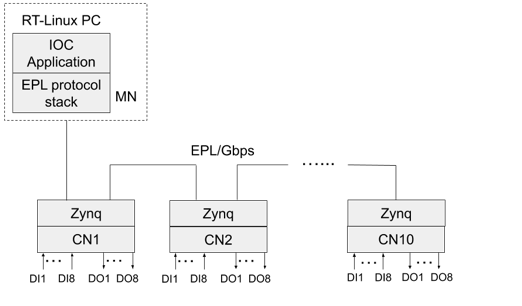
\includegraphics[width=0.8\textwidth]{design1-arch.png}
  \caption{方案1系统硬件架构图}
  \label{fig:design1-arch}
\end{figure}


\begin{itemize}

\item \textbf{方案2} \\ 
方案2所设计的系统架构图~\ref{fig:design2-arch}如所示,与方案1不同的是,主站与从站均是基于FPGA的控制器,IOC应用程序运行在PC上,IOC应用程序通过千兆以太网与主站通信。

\begin{figure}[!htb]
  \centering
  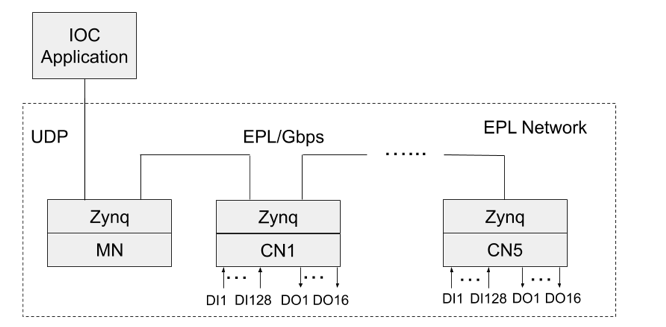
\includegraphics[width=0.8\textwidth]{design2-arch.png}
  \caption{方案2系统硬件架构图}
  \label{fig:design2-arch}
\end{figure}

\end{itemize}

\subsection{EPICS设备驱动程序的开发}

EPICS设备驱动程序的功能是将POWERLINK网络中传输的数据转换为EPICS IOC中各种记录(Record)。EPICS IOC的软件结构如图~\ref{fig:design1-driver-arch}中“IOC Application”部分所示,IOC以运行时数据库(Runtime Database)为核心,运行时数据库由记录(Record)组成,记录中保存着与IO信号有关的所有数据,如信号的值、工程单位、处理时间、报警范围等。记录通过Record Support、Device Support及Driver Support来与硬件设备交换信息。

驱动程序的开发工作主要是按照EPICS的接口规范来编写Device Support,Driver Support负责与POWERLINK网络通信。具体来说,IOC应用程序与POWERLINK网络中的主站建立通信,以获取POWERLINK网络中各从站的IO数据。IOC的任务是监控POWERLINK网络中各节点的状态,所以IOC与POWERLINK主站之间的通讯实时性要求并不高。在方案1所设计的系统里,oplk和IOC作为两个应用程序运行在同一台PC上,所以我们采用基于进程间Socket(IPC Socket)的通信方式来实现IOC与POWERLINK主站的通信。

\begin{figure}[!htb]
  \centering
  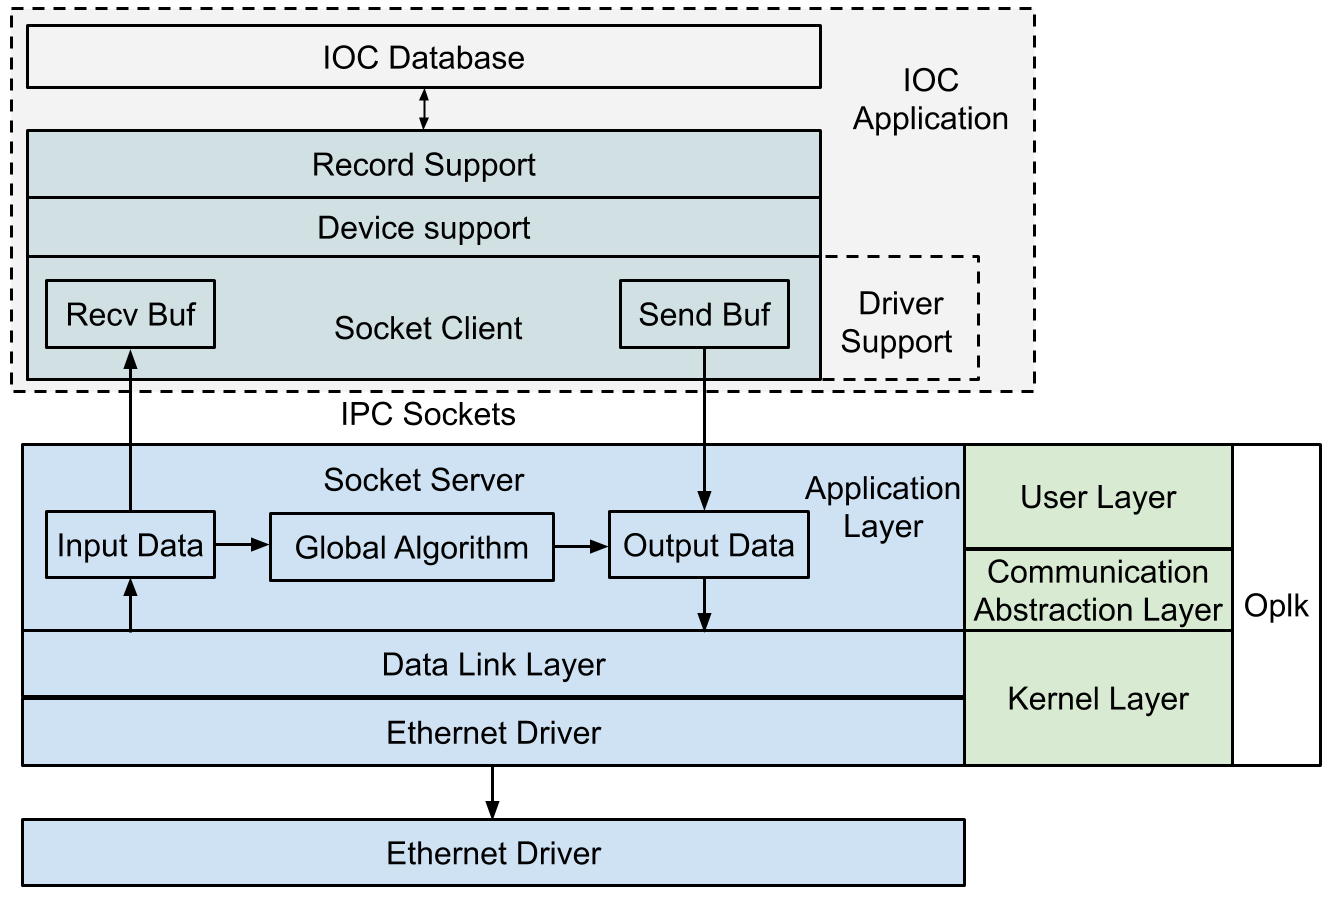
\includegraphics[width=\textwidth]{design1-driver-arch.png}
  \caption{方案1主站的软件架构图}
  \label{fig:design1-driver-arch}
\end{figure}

主站的软件架构如图~\ref{fig:design1-driver-arch}所示,由oplk和IOC应用程序组成。oplk通过“Data Link Layer”收集各从站的DI信号,这些信号被发送到“Application Layer”中名为“Input Data”缓存区中。同时作为Socket服务端,“Application Layer”会将“Input Data”缓存区中的数据传输到IOC应用程序。“Application Layer”中名为“Output Data”的缓存区用于接收来自IOC应用程序的控制参数等命令,并向下将控制参数发送到相应的从站。

IOC中的EPICS驱动程序由“Driver Support”和“Device Support”组成。作为Socket客户端,“Driver support”中有两个缓存区,用于存储与oplk程序交换的数据。在这些缓存区中,“Recv Buf”缓存区用于接收来自oplk程序的数据,“Send Buf”缓存区用于存储发送至oplk程序的控制参数。“Device Support”的功能是将两个缓存区中的数据转化成EPICS中的记录,目前“Device Support”支持标准的EPICS DI和DO记录。

\begin{itemize}

\item \textbf{方案2} \\ 
在方案2所设计的系统里,主站是一台基于FPGA的控制器,IOC应用程序运行在一台PC上,主站和pc之间的通讯基于UDP socket的方式实现,方案2所设计的软件系统架构~\ref{fig:design2-driver-arch}如所示。总体设计与方案一相似,不同点是主站POWERLINK协议的应用层是UDP客户端,IOC应用程序是UDP服务端,通信物理层采用千兆以太网。

\begin{figure}[!htb]
  \centering
  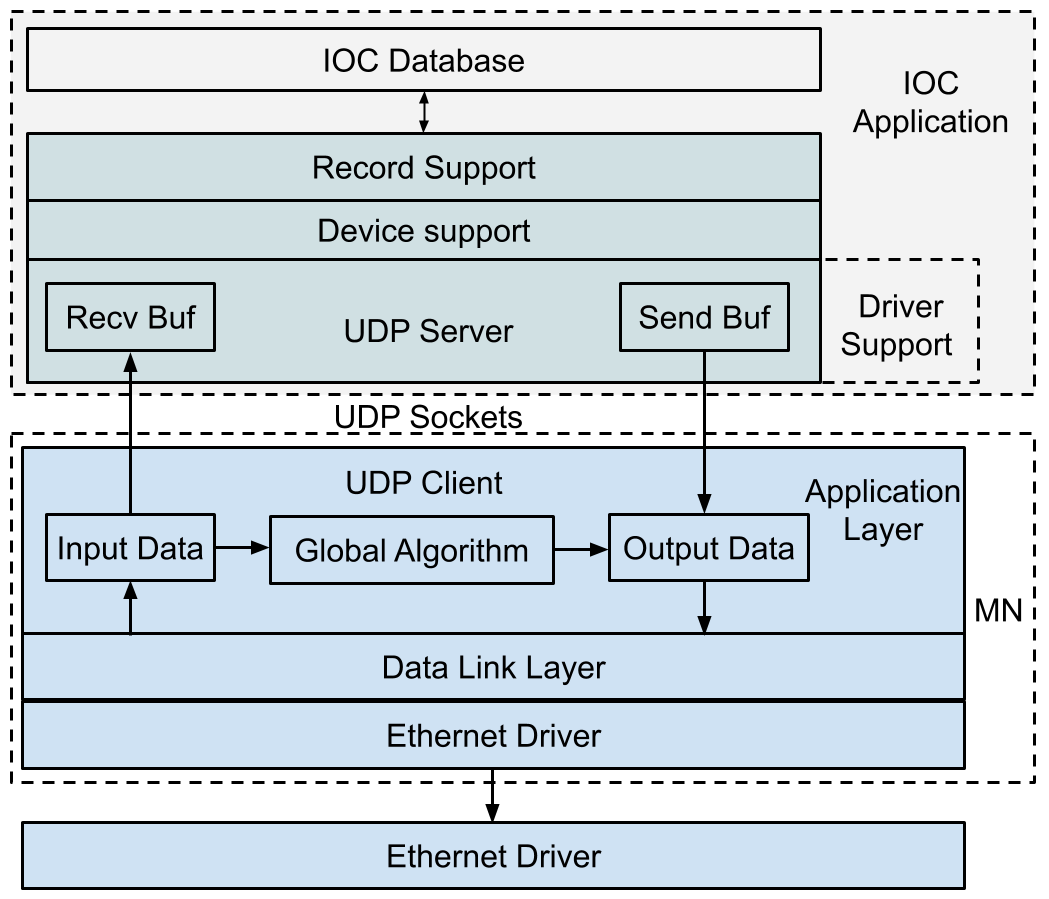
\includegraphics[width=\textwidth]{design2-driver-arch.png}
  \caption{方案2EPICS设备驱动软件架构图}
  \label{fig:design2-driver-arch}
\end{figure}

\end{itemize}

\subsection{基于FPGA的前端控制器的设计与开发}

FPGA平台具有较高的实时性和灵活性,是实现POWERLINK协议较为理想的平台,也是目前普遍采用的方式。基于FPGA实现POWERLINK的方案有两种,方案1是在FPGA中通过软核的形式来运行openPOWERLINK程序,方案2是采用纯硬件描述语言Verilog HDL来实现POWERLINK的协议栈。具体来说,方案2可以采用POWERLINK协议分离的方式来实现,数据链路层、物理层基于FPGA来实现,应用层基于ARM核来实现。这种设计既可以通过FPGA来达到较高的硬实时性,又可以利用ARM系统来兼容各种应用层协议。

方案1的技术细节和性能测试已在~\ref{subsection:基于FPGA实现POWERLINK协议}中详细介绍,对比方案1,方案2有以下特点和性能优势:

\begin{enumerate}
  \item 采用硬件语言Verilog HDL来实现,无需软核,无需外扩RAM,即可以达到硬实时的性能。
  \item 实时性高,最短通信周期可以到达到几十$\mu$s,抖动可以达到数十ns。若采用MCU软核的方式,很难达到这样的性能指标。
  \item 对比~\ref{subsection:基于FPGA实现POWERLINK协议}中方案1的通信过程,方案2使用硬件加速,在FPGA中实现自动回复功能。当PReq数据帧进入到FPGA中的MAC时,MAC会将准备好的上一周期的PRes数据快速发送 到网络上。当使用了自动回复功能后,PReq数据桢和PRes数据帧之间的时间间隔可以达到几个$\mu$s,从而缩短通信周期,提高实时性。
  \item 兼容不同的应用层。虽然标准POWERLINK协议的应用层为CANopen,但是不同行业有不同的标准和习惯。采用此方案,可以仅使用Verilog HDL实现的数据链路层,而自定义应用层的协议。
  \item 兼容不同的物理层。在保持数据链路层一致的情况下,此方案可以满足100Mbps、1000Mbps以太网。
\end{enumerate}

\subsubsection{硬件介绍}

\begin{figure}[!htb]
  \centering
  \includegraphics[width=\textwidth]{Zynq-arch.png}
  \caption{Xilinux Zynq-7000芯片的架构图}
  \label{fig:Zynq-arch}
\end{figure}

在核心片的选择上,采用Xilinux Zynq-7000型号的芯片来实现POWERLINK协议。该芯片的结构如图~\ref{fig:Zynq-arch}所示,Zynq-7000器件在硬件上配备了双核ARM Cortex-A9处理器,该处理器与基于28nm Artix-7的可编程逻辑集成,在软件上兼具ARM处理器的软件可编程性与FPGA的硬件可编程性。由于其高度的灵活性和较小的硬件占用空间,Zynq是自动化项目中小型高性能设备的理想平台。我们可以利用Zynq芯片的ARM处理器实现POWERLINK协议的应用层,利用FPGA实现POWERLINK协议的数据链路层和物理层,从而达到硬实时的性能。

\begin{figure}[!htb]
  \centering
  
\includegraphics[width=\textwidth]{zynq-core-board-arch.png}
  \caption{基于Zynq的核心板硬件架构图}
  \label{fig:zynq-core-board-arch}
\end{figure}

\begin{figure}[!htb]
  \centering
  
\includegraphics[width=\textwidth]{zynq-floor-arch.png}
  \caption{基于Zynq的底板硬件架构图}
  \label{fig:zynq-floor-arch}
\end{figure}

基于核心片Zynq,设计了由核心板和底板组成的控制器,核心板通过相应引脚与底板相连接,核心板的硬件架构如图~\ref{fig:zynq-core-board-arch}所示,底板的硬件架构如图~\ref{fig:zynq-floor-arch}所示,核心板硬件系统的各部分为:

\begin{enumerate}
  \item 核心片:POWERLINK网络通信的核心部件,选用Xilinux Zynq-7000家族的芯片,具体型号为XC7Z020,逻辑单元数85k。

  \item 外部存储:外部存储连接到ARM硬核上,包括512MB的DDR3、16MB的Qspi$\_$Flash、4GB的EMMC和TF$\_$CARD,用来提供POWERLINK程序的运行空间和存储空间。

  \item Reset$\&$WatchDog:外置看门狗计时器,用来复位程序。

  \item Gig$\_$Ethernet:千兆以太网PHY芯片,通过此以太网接口与EPICS IOC应用程序程序通信。

  \item JTAG接口:POWERLINK协议程序的下载和调试接口。
 
  \item Expansion IO:扩展IO引脚,用于连接底板。
\end{enumerate}

底板硬件系统的各部分为:

\begin{enumerate}
  \item POWERLINK×2:用于POWERLINK通信的HUB的两个千兆以太网接口。

  \item GPIOs:提供DI、DO接口。

  \item 本地通讯接口:提供了RS232、RS484以及CAN本地通讯接口。
\end{enumerate}

图~\ref{fig:zynq-board-photo}所示的是控制器电路板实物,可从照片中看出GPIO接口、两个POWERLINK网口。

\begin{figure}[!htb]
  \centering
  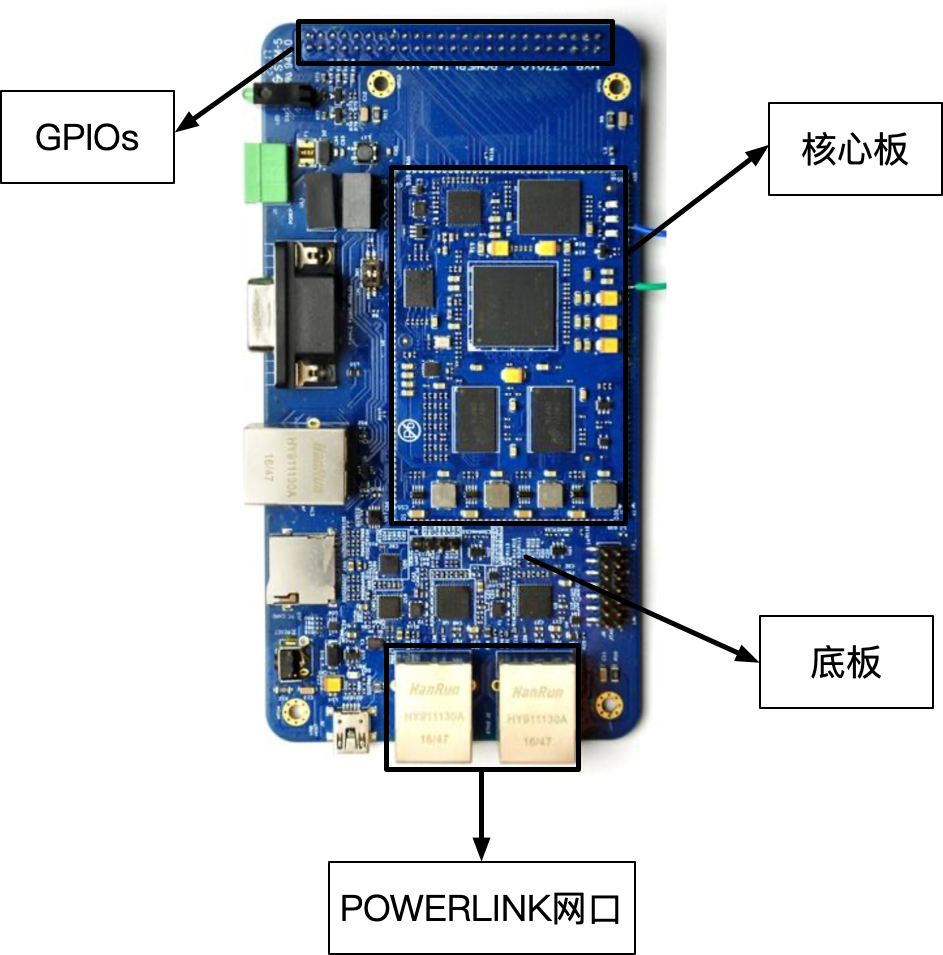
\includegraphics[width=0.8\textwidth]{design1-board-photo.png}
  \caption{控制器电路板照片}
  \label{fig:design1-board-photo}
\end{figure}

\begin{figure}[!htb]
  \centering
  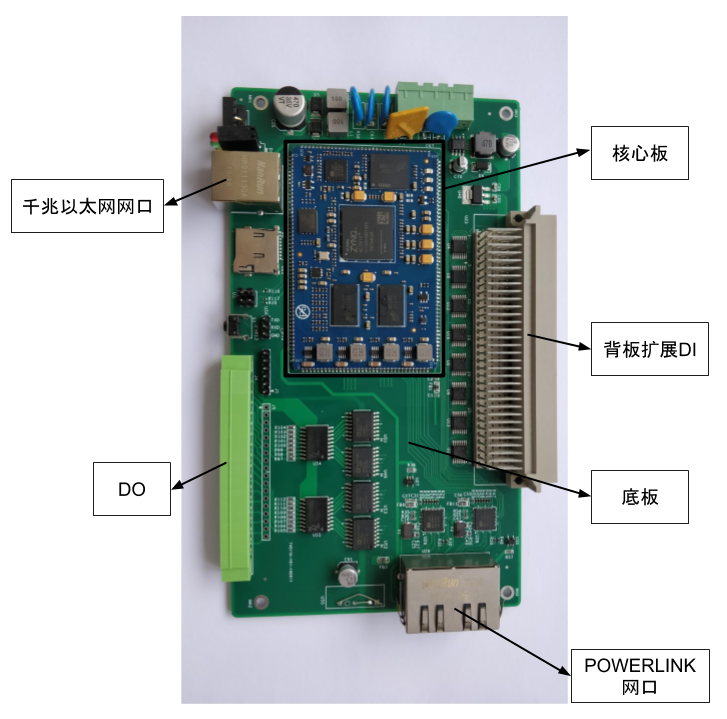
\includegraphics[width=\textwidth]{zynq-board-photo.png}
  \caption{控制器电路板照片}
  \label{fig:zynq-board-photo}
\end{figure}

\subsubsection{软件设计}

基于Zynq的硬件架构,设计了如图~\ref{fig:design1-zynq-software}所示的软件架构,首先介绍与POWERLINK通信有关的软件设计。从站POWERLINK协议的软件架构由三部分组成:基于ARM处理器的POWERLINK应用层、基于FPGA的POWERLINK数据链路层和物理层。

\begin{figure}[!htb]
  \centering
  \includegraphics[width=\textwidth]{Zynq-EPL-arch.png}
  \caption{基于Zynq的控制器软件架构图}
  \label{fig:Zynq-EPL-arch}
\end{figure}

\begin{figure}[!htb]
  \centering
  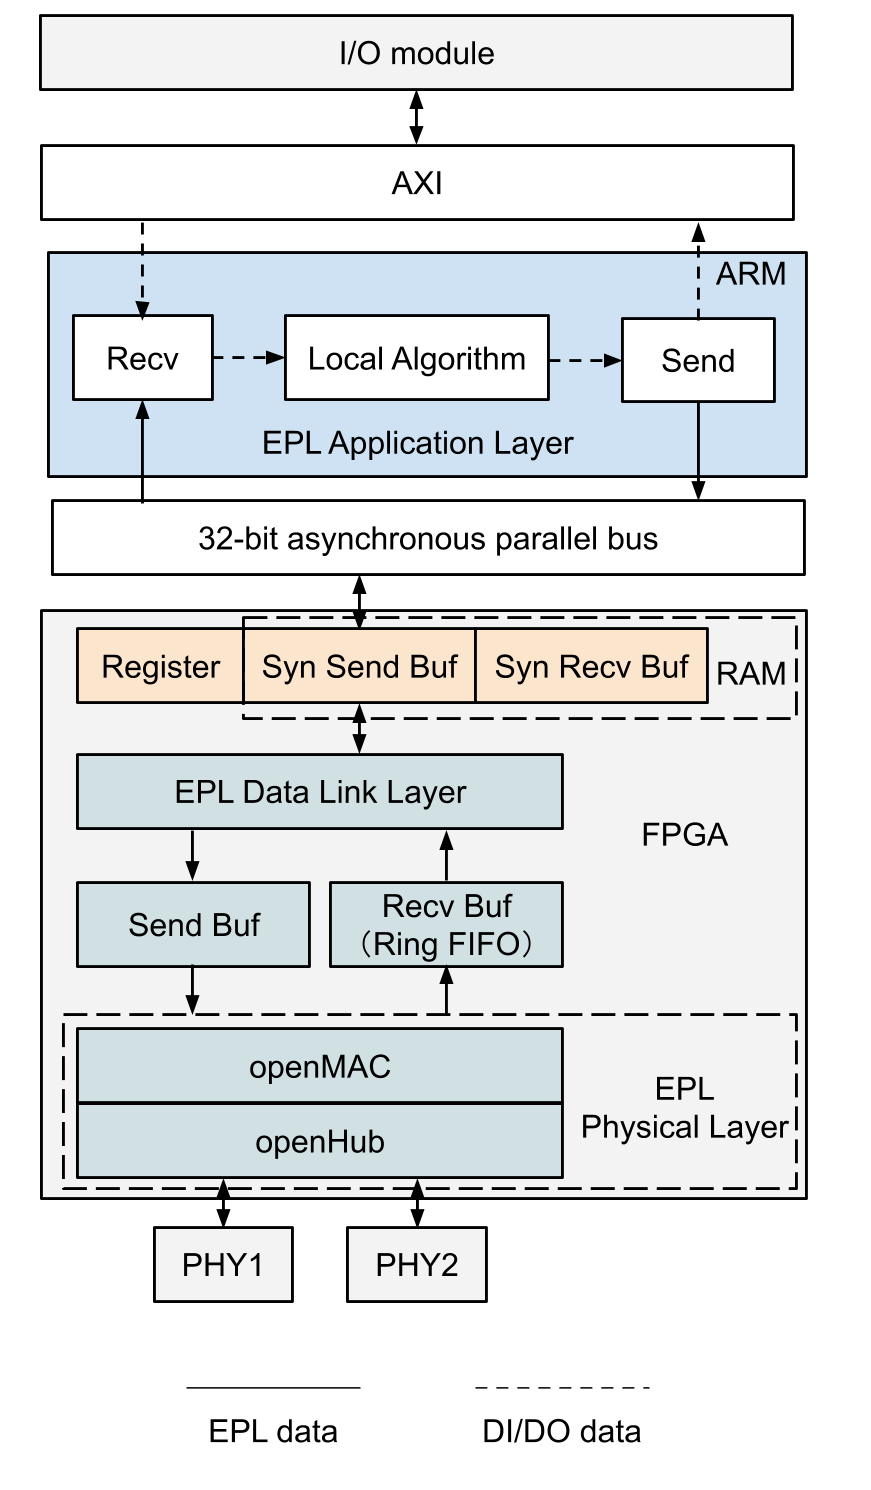
\includegraphics[width=\textwidth]{design1-zynq-software.png}
  \caption{基于Zynq的控制器软件架构图}
  \label{fig:design1-zynq-software}
\end{figure}

\begin{itemize}

\item \textbf{物理层} \\ 
POWERLINK物理层采用Verilog HDL实现,由openHub和openMAC两部分组成。openMAC支持千兆以太网PHY芯片,双口openHUB可以以菊花链的形式来连接两个相邻的从站。 

\item \textbf{数据链路层} \\ 
POWERLINK的数据链路层状态机和NMT网络管理等采用Verilog HDL来实现。

\item \textbf{应用层} \\ 
POWERLINK协议的应用层基于ARM架构采用C语言实现。除了可以使用标准POWERLINK的CANopen应用层以外,还支持其他任意的应用层。

\item \textbf{API接口} \\ 
应用层与数据链路层之间的接口为API接口。该接口采用寄存器和双口RAM实现,应用层通过32位并行总线来访问寄存器和双口RAM中的数据。

\end{itemize}

数据传输的流程和细节如下:

\begin{enumerate}
  \item POWERLINK应用层通过32位并行总线将数据写入寄存器和“Syn Buf”缓存区,缓存区采用双口RAM实现从而避免数据链路层和应用层同时对RAM操作造成的冲突。

  \item 在数据链路层和应用层之间,有“Sync Recv Buf”和“Sync Send Buf”两个缓存区,分别用于保存数据链路层收到的同步数据和下个周期要发送的同步数据。同步数据是周期性传输的数据,在每个周期开始的时候,数据链路层都会给应用层一个同步中断信号,触发应用层的同步回调函数对“Sync Send Buf”和“Sync Recv Buf”两个缓存区中的数据进行读写操作。

  \item 数据链路层组建要发送的数据包,并写入MAC层的“Send Buf”缓存区中,然后启动发送。发送完成,通过寄存器的标志位来反馈发送是否正确。

  \item MAC层接收到数据时,将其放到MAC层的“Recv Buf”缓存区中,该缓存区为环形,可以存放2个最大以太网的帧。当收到一个完整且正确的PReq数据帧,即该数据帧的目标节点号与本节点相同,则通知数据链路层进行处理,将数据帧的有效数据部分从MAC的“Recv Buf”拷贝到“Sync Recv Buf”中。如果接收到的数据有问题,则丢弃本帧数据,并将重新设置MAC的接收设置,为下一次接收做准备。当处理完毕,通知MAC层释放接收缓冲区“Recv Buf”,用来保存后面的数据帧。
 
\end{enumerate}

除了完成POWERLINK协议通信,从站还需要完成IO信号的采集与输出。如图~\ref{fig:Zynq-EPL-arch}所示,FPGA中的RAM存储IO模块的数据,应用层可以直接通过RAM实现对DI/DO信号的操作。

主站的POWERLINK通信协议的实现与从站相同,除此之外,如图~\ref{fig:design2-driver-arch}所示,主站的应用层需要实现一个UDP客户端。

\subsection{原型系统搭建}

为测试基于POWERLINK的EPICS分布式IO控制系统的性能,基于第~\ref{section:原型系统性能测试}节提出的两种系统架构设计,我们分别搭建了两套原型系统,以下将分别介绍两套原型系统的硬件组成和软件开发。

\subsection{方案1原型系统硬件组成} 

按照第~\ref{section:原型系统性能测试}节提出的方案1,我们搭建了如图~\ref{fig:prototype-mn-pc-photo}所示的原型系统。照片上可以看到1台PC和10台FPGA控制器。

\begin{figure}[!htb]
  \centering
  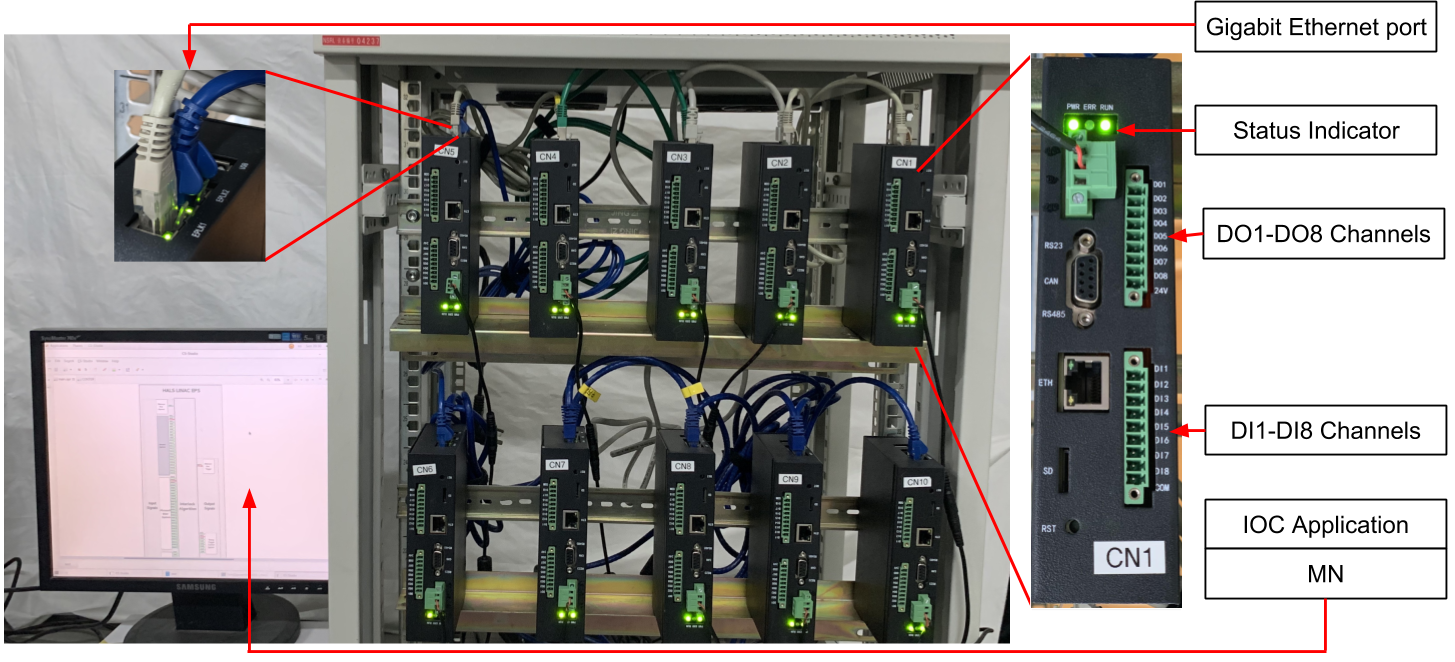
\includegraphics[width=\textwidth]{prototype-mn-pc-photo.png}
  \caption{基于方案1的原型系统照片}
  \label{fig:prototype-mn-pc-photo}
\end{figure}

\subsubsection{EPICS IOC以及POWERLINK主站的搭建}

EPICS IOC应用程序和openPOWERLINK主站程序运行在在同一台PC上,PC上安装了带有内核实时补丁3.10的Centos7系统。该PC的网卡型号为intel 82573,openPOWERLINK主站程序通过该网卡驱动,运行在在内核模式下。

\subsubsection{基于Zynq的前端控制器}

原型系统共有10个从站,每个从站都是基于Zynq的控制器。控制器对外提供了8个DI和8个DO通道,DI接口如图~\ref{fig:zynq-8di-interface}所示,公共端(COM0端口供DI输入使用,输入设备的地需要与此处共地形成回路;DO接口如图~\ref{fig:zynq-8do-interface}所示,为源型输出,24V输入端为DO输出负载所接的正24V电压。另外,2个千兆以太网端口用于连接相邻的从站,3个状态指示灯分别显示控制器的电源状态,错误状态和操作状态,灯亮表示状态正常。

\begin{figure}[!htb]
  \centering
  
\includegraphics[width=\textwidth]{zynq-8di-interface.png}
  \caption{方案1从站控制器DI接口}
  \label{fig:zynq-8di-interface}
\end{figure}

\begin{figure}[!htb]
  \centering
  
\includegraphics[width=\textwidth]{zynq-8do-interface.png}
  \caption{方案1从站控制器DO接口}
  \label{fig:zynq-8do-interface}
\end{figure}

\subsubsection{POWERLINK网络搭建}

原型系统基于千兆POWERLINK网络搭建,各从站按照节点号从小到大的顺序依次相连成直线拓扑。

\subsection{方案2原型系统硬件组成} 

按照第~\ref{section:原型系统性能测试}节提出的方案2,我们搭建了如图~\ref{fig:prototype-mn-fpga-photo}所示的原型系统。照片上可以看到1台PC和6台FPGA控制器,EPICS IOC应用程序运行在PC上,6台控制器组成了千兆POWERLINK网络,其中1台为主站,5台为从站,各从站按照节点号从小到大的顺序依次相连成直线拓扑。

\begin{figure}[!htb]
  \centering
  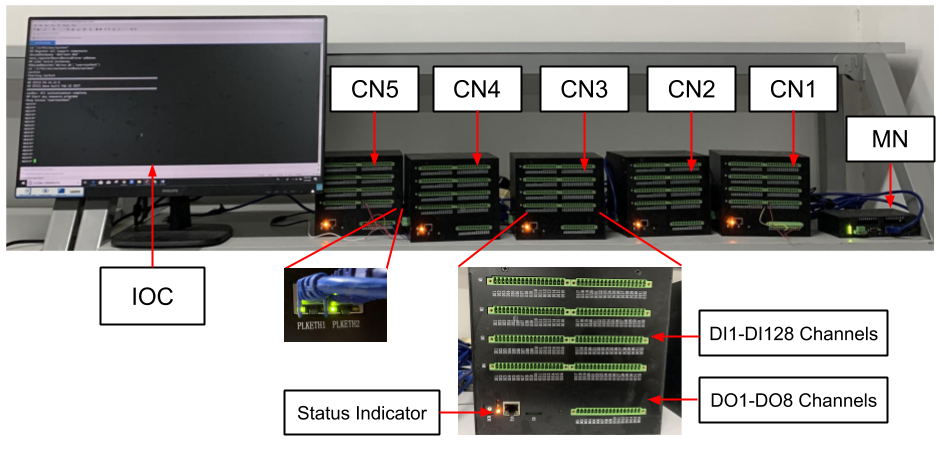
\includegraphics[width=\textwidth]{prototype-mn-fpga-photo.png}
  \caption{基于方案2的原型系统照片}
  \label{fig:prototype-mn-fpga-photo}
\end{figure}

\subsubsection{基于Zynq的POWERLINK主站}

主站是基于Zynq的控制器,除了提供POWERLINK网络接口外,还提供一个千兆以太网接口与PC上的IOC应用程序通信。

\subsubsection{基于Zynq的POWERLINK从站}

每个从站都是基于Zynq的控制器,控制器对外提供128个DI和32个DO通道,DI接口如图~\ref{fig:zynq-16di-interface}所示,为漏型输入;DO接口如图~\ref{fig:zynq-16do-interface}所示,为源型输出。因为Zynq芯片上的引脚有限,如图~\ref{fig:Zynq-EPL-arch}所示,我们采用数据选择器(Data Selector)来扩展DI数量。

\begin{figure}[!htb]
  \centering
  
\includegraphics[width=\textwidth]{zynq-16di-interface.png}
  \caption{方案2从站控制器DI接口}
  \label{fig:zynq-16di-interface}
\end{figure}

\begin{figure}[!htb]
  \centering
  
\includegraphics[width=\textwidth]{zynq-16do-interface.png}
  \caption{方案2从站控制器DO接口}
  \label{fig:zynq-16do-interface}
\end{figure}

\subsection{原型系统软件开发}

\label{subsection:原型系统软件开发}

原型系统的软件开发包括EPICS IOC应用程序和Zynq控制器程序的开发。方案1和方案2中EPICS IOC应用程序的开发按照图~\ref{fig:design1-driver-arch}和图~\ref{fig:design2-driver-arch}所示的软件架构开发。另外在主站的POWERLINK应用层加入了全局算法功能,主站通过全局算法处理来自各从站控制器的DI信号,并通过相应的从站输出相应DO信号。基于Zynq的从站控制器程序按照图~\ref{fig:Zynq-EPL-arch}所示的软件架构开发,除了完成POWERLINK通信以外,在POWERLINK应用层加入了本地算法功能,从站控制器可以直接对DI信号进行处理,并输出相应DO信号。以下是Zynq控制器的程序框架:
\begin{lstlisting}
while(1)
{ 
  //处理出来POWERLINK网络状态机跳转,网络配置等
  ret = oplk_process();

  //主站UDP Client通信程序
  udp_send_data((const char *) UDP_TX_Buffer, int data_len);
  udp_recieve_data(const char *frame, int data_len);

  //从站读写DI/DO和本地算法程序
  CHA_DI_read(u32 Input_Pin);
  local_process_data;
  FPGA_DO_write(u32 Output_Pin, u32 Data);
}

//同步回调函数,由SoC触发
void syncCb(void)
{
  //负责读写同步数据和主站全局算法程序
  pdou_copyRxPdoToPi();
  global_process_data();
  pdou_copyTxPdoFromPi();
}
\end{lstlisting}

程序主要由while循环程序和POWERLINK通信同步回调函数组成。while循环程序一直运行,用来处理POWERLINK异步事件,状态机跳转,网络配置等,对于主站我们在while循环程序里添加了UDP Client程序;对于从站,我们在while循环程序里添加了DI/DO读写和和本地算法程序。通信同步回调函数“synCb()”由SoC触发,用于处理周期性同步数据,对于主站,我们在此添加了全局算法程序。


\section{原型系统性能测试}

\label{section:原型系统性能测试}

对于原型系统来说,powerlink网络实时性能。不考虑上位机我们对两套原型系统进行了一系列测试,其中包括通信周期、响应时间的实时性能,下面将详细介绍测试细节和测试结果。

\subsection{通信周期测试}

\begin{figure}[!htb]
  \centering
  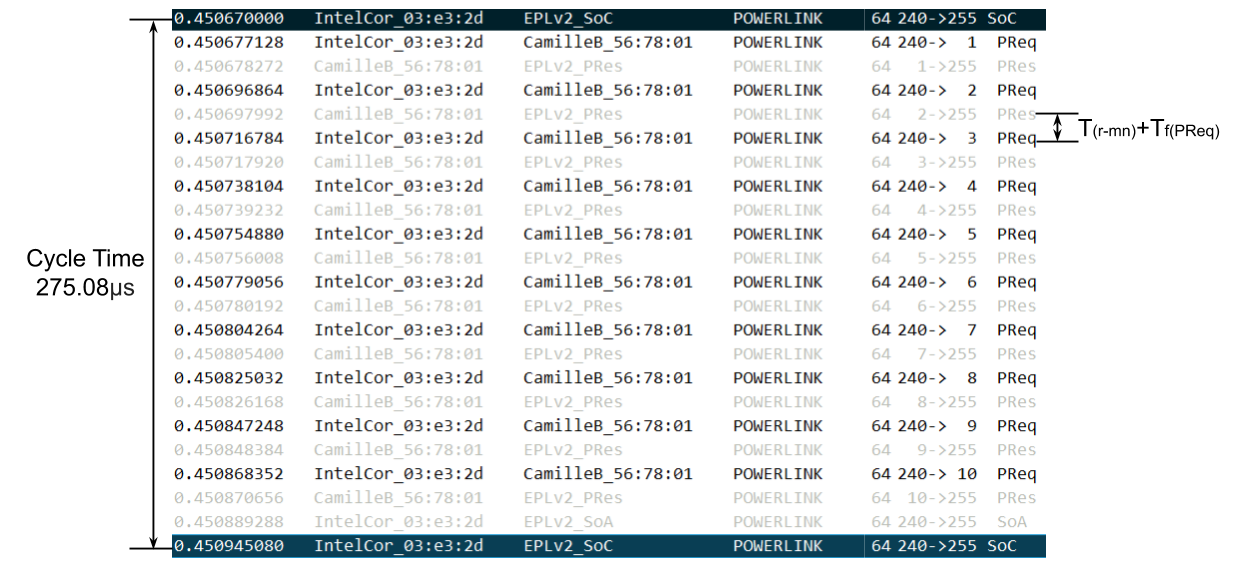
\includegraphics[width=\textwidth]{design1-cycle-time-test.png}
  \caption{方案1POWERLINK数据帧抓取结果}
  \label{fig:design1-cycle-time-test}
\end{figure}

\begin{figure}[!htb]
  \centering
  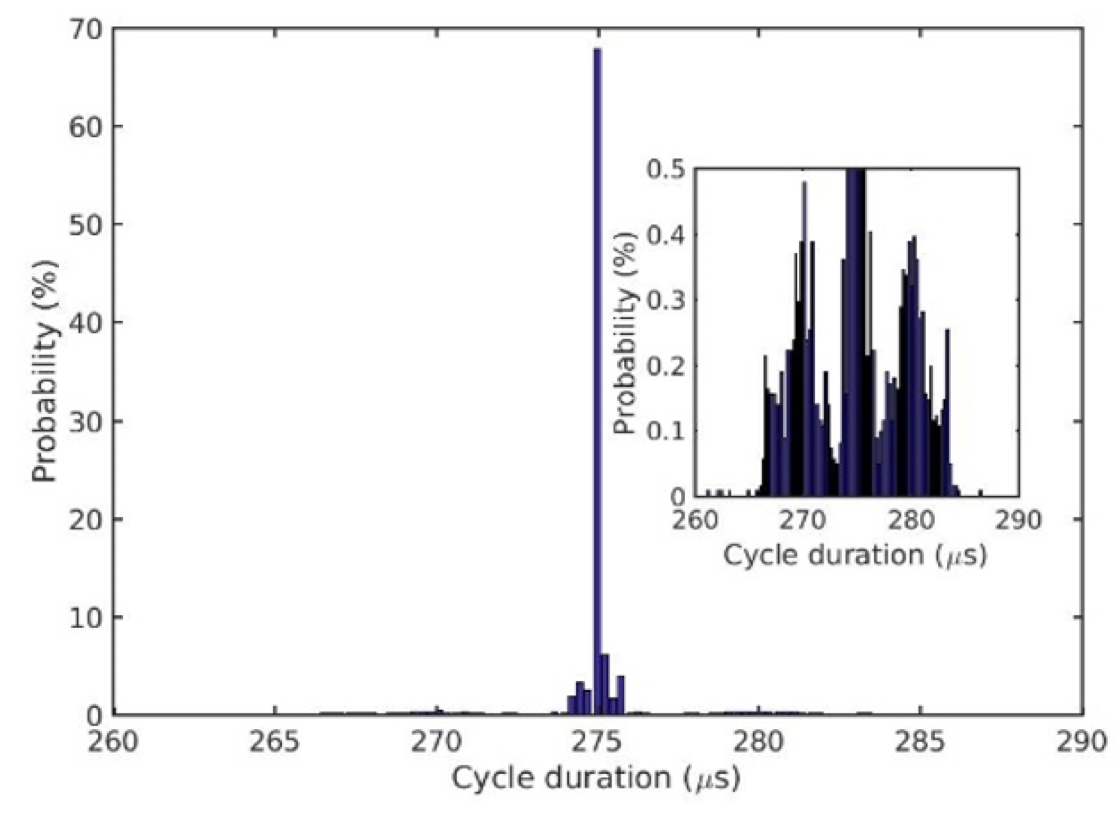
\includegraphics[width=\textwidth]{design1-cycle-time-density.png}
  \caption{方案1POWERLINK通信周期概率密度分布}
  \label{fig:design1-cycle-time-density}
\end{figure}

通信周期是衡量实时系统性能的重要参数,短时间周期内持续稳定运行对于实时性系统至关重要。我们使用openCONFIGURATOR网络组态工具来配置不同的POWERLINK通信周期,利用ProfiShark 1G Ethernet Troubleshooter以太网诊断工具来测试原型系统在不同通信周期下的运行情况,从而确定系统最短通信周期。ProfiShark 1G是一款专用于千兆以太网监测的故障诊断仪,硬件时间戳仅为8ns,可以抓取高实时性的POWERLINK通信数据,将抓包结果输出为可被Wireshark解析的pcap格式文件。

我们对分别对方案1和方案2原型系统进行了通信周期测试,测试结果如下:

\subsubsection{方案1测试结果:}
图~\ref{fig:design1-cycle-time-test}所示的是方案1原型系统的数据帧抓取结果,通信周期可根据两个连续SoC帧之间的时间隔计算得出的,如图~\ref{fig:design1-cycle-time-test}所示。我们抓取来超过12k个连续的POWERLINK帧,并将通信周期的概率密度分布绘制在图~\ref{fig:design1-cycle-time-density}中。图~\ref{fig:design1-cycle-time-density}表明,大多数情况下的通信周期都非常接近系统的通信周期设定值275$\mu$s,通信周期周期的最大偏移约为12$\mu$s。

\subsubsection{方案2测试结果:}
方案2原型系统的通信周期最快可配置为50$\mu$s,50$\mu$s通信周期下的通信过程如图~\ref{fig:design2-cycle-time-test}所示。我们抓取了超过20k个连续的POWERLINK数据帧,并将通信周期的概率密度分布绘制在图~\ref{fig:design2-cycle-time-density}中。该图显示大多数情况下的通信周期为50.024$\mu$s,少数情况为50.016$\mu$s和50.032$\mu$s,此结果是由基于zynq的控制器和ProfiShark 1G以太网分析仪的125Mhz时钟频率引起的。通信周期周期的最大偏移仅为32$\mu$s,抖动非常小。

\begin{figure}[!htb]
  \centering
  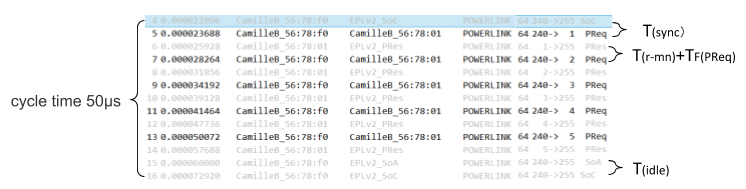
\includegraphics[width=\textwidth]{design2-cycle-time-test.png}
  \caption{方案2POWERLINK数据帧抓取结果}
  \label{fig:design2-cycle-time-test}
\end{figure}

\begin{figure}[!htb]
  \centering
  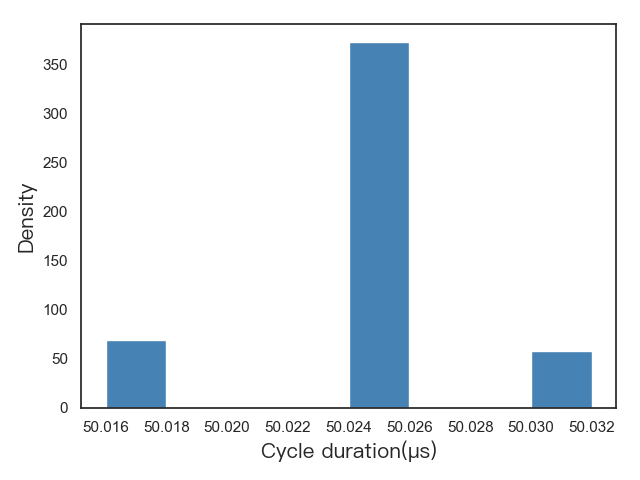
\includegraphics[width=\textwidth]{design2-cycle-time-density.png}
  \caption{方案2POWERLINK通信周期概率密度分布}
  \label{fig:design2-cycle-time-density}
\end{figure}

\subsection{响应时间测试}
响应时间是衡量系统实时性能的重要参数。在我们的测试中,响应时间是指DI信号到达系统与系统输出DO信号之间的时间间隔。原型系统中具有本地响应和全局响应两种响应机制,本地响应指是从站本身对于DI信号直接做出的响应,全局响应是指DI信号经过POWERLINK网络传输,被主站处理之后,系统做出的响应。我们分别对方案1和方案2原型系统进行了本地响应时间和全局响应时间的测试,测试结果和分析如下:

\subsubsection{方案1原型系统响应时间测试:}

我们首先对从站控制器进行本地响应时间的测量,本地响应的过程如下:\\
1.原型系统的GPIO读取输入信号,并将输入值以二进制形式存储在FPGA的双口RAM中;\\
2.ARM通过32bit并行总线读取并处理RAM中的输入数据;\\
3.处理结果通过32bit并行总线写入相应的RAM中并通过GPIO输出信号。\\

我们将1号从站控制器的输入和输出信号连接到示波器上,以输入和输出信号的上升沿时间差来表示本地响应时间。测试结果如图~\ref{fig:design1-local-response-time}所示,Ch1(黑线)代表1号从站控制器的输入信号; Ch2(青色线)代表1号从站控制器的输出信号,响应时间约为400$\mu$s。这个时间延迟包括从站控制器输入/输出接口电路中的光电耦合器的延时和ARM读取处理数据的时间。由于ARM的时钟频率为125MHz,ARM读取处理数据的时间仅在$\mu$s量级,所以本地响应时间主要是光电耦合器延导致的延时。
\begin{figure}[!htb]
  \centering
  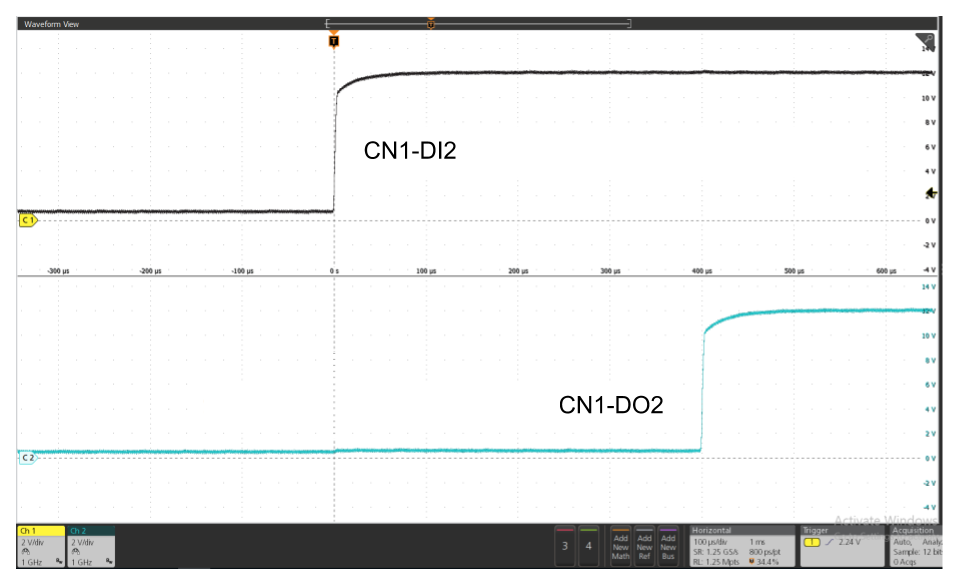
\includegraphics[width=\textwidth]{design1-local-response-time.png}
  \caption{方案1原型系统本地响应时间测试结果}
  \label{fig:design1-local-response-time}
\end{figure}

全局响应时间由从站光电耦合器的延迟和POWERLINK网络通信时间组成。通信时间包括用于封装和解封装数据帧的时间、主站处理数据的时间、电缆中数据传输的时间以及HUB中的时间延迟。在全局响应时间的测试中,我们设计了如图~\ref{fig:design1-response-process}所示的响应过程。在第n个周期,1号从站的输入信号通过PRes数据帧进入POWERLINK网络,$T_{cn1-di1}$为1号从站接收到输入信号的时刻,该信号经过主站处理之后,处理结果在第n+1个周期通过PReq数据帧从10号从站输出,$T_{cn10-do1}$为10号从站输出信号的时刻。该响应过程经历两个连续周期,$T_{com}$是此过程的通信时间。根据POWERLINK通信顺序,10号从站是通信周期中的最后一个参与通信的。因此,$T_{com}$也是该系统全局响应的最长通信时间。如图~\ref{fig:design1-cycle-time-test}所示,可以使用ProfiShark 1G以太网分析仪捕获数据帧来计算$T_{com}$,大约为457$\mu$s。示波器测得的总响应时间如图~\ref{fig:design1-response-time-result}所示,Ch1(黑线)代表1号从站控制器的输入信号; Ch3(红色线)代表10号从站控制器的输出信号,响应时间约为870$\mu$ss。考虑到在本地响应过程光电耦合器引起的延迟时间约为400$\mu$s,其他因素引起的延迟约为21$\mu$s。

\begin{figure}[!htb]
  \centering
  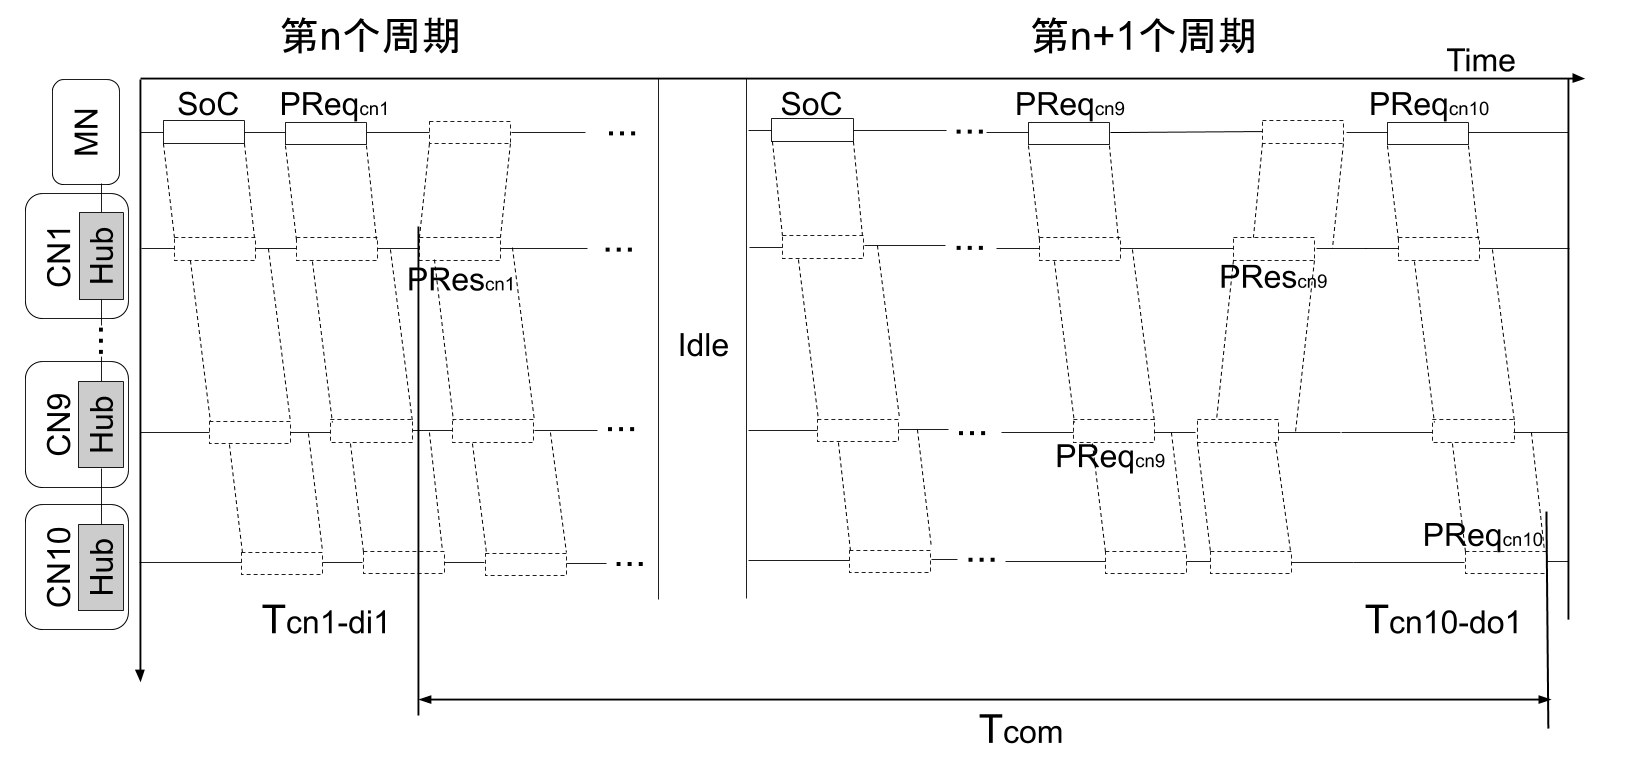
\includegraphics[width=\textwidth]{design1-response-process.png}
  \caption{方案1原型系统全局响应过程}
  \label{fig:design1-response-process}
\end{figure}

\begin{figure}[!htb]
  \centering
  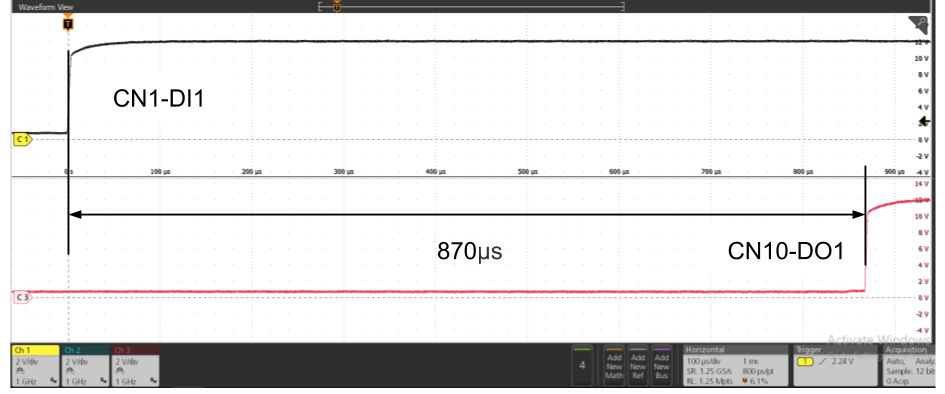
\includegraphics[width=\textwidth]{design1-response-time-result.png}
  \caption{方案1原型系统全局响应时间测试结果}
  \label{fig:design1-response-time-result}
\end{figure}

\subsubsection{方案2原型系统响应时间测试:}

我们首先选择原型系统中的5号从站控制器进行了本地响应时间测量,同样以输入和输出信号的上升沿时间差来表示本地响应时间。测试结果如图~\ref{fig:design2-local-response-time}所示,Ch2(青色线)代表5号从站控制器的输入信号;Ch3(青色线)代表5号从站控制器的输出信号,响应时间为5$\mu$s。本地响应时间延迟主要是由从站控制器输入/输出接口电路中的磁耦合器造成的,我们采用的是型号为ADuM140x1是高速磁耦合器,较之方案1的光耦合器可以大大提高信号传输速率。

\begin{figure}[!htb]
  \centering
  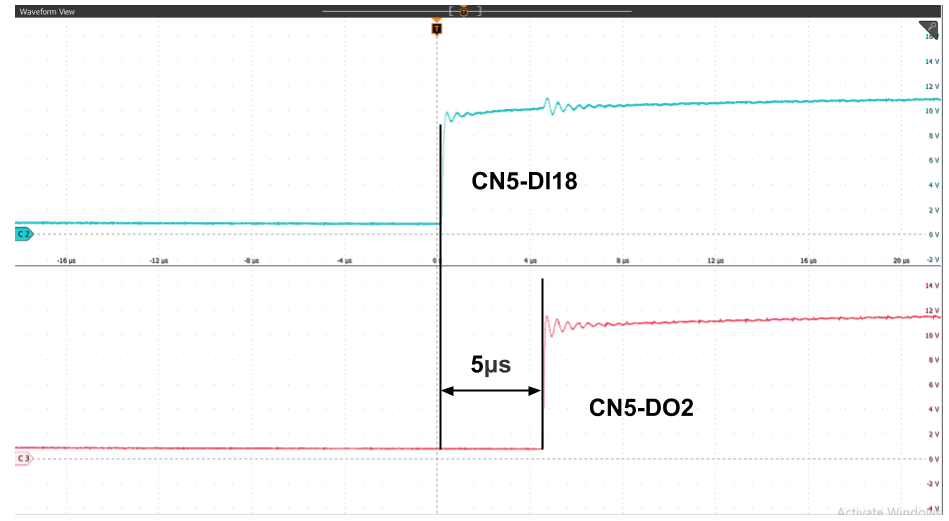
\includegraphics[width=\textwidth]{design2-local-response-time.png}
  \caption{方案2原型系统本地响应时间测试结果}
  \label{fig:design2-local-response-time}
\end{figure}

方案中2原型系统的全局响应时间($T_{global-response}$)由POWERLINK网络通信时间($T_{powerlink}$)和从站处理输入信号($T_{CN-process}$)的时间组成,见公式~\ref{equation1} 。在全局响应时间的测试中,我们设计了如图~\ref{fig:design2-response-process}所示的响应过程。在第n个周期,1号从站的输入信号通过PRes数据帧进入POWERLINK网络,$T_{cn1-di1}$为1号从站接收到输入信号的时刻,在第n+1个周期主站对该输入信号进行处理,处理结果在第n+2个周期通过PReq数据帧从5号从站输出,$T_{cn5-do1}$为5号从站输出信号的时刻。与方案1通信过程不同的是,该响应过程需要经历三个连续周期,原因是主站对输入信号的处理时间为数$\mu$s,无法在本周期将处理结果传输出去。具体解释如下:在第n+2的周期开始的时候,主站发送SoC数据帧后产生同步中断信号,中断信号会触发应用层的同步回调函数“synCb( )”对“Sync Recv Buf”缓存区中的输入数据进行处理,这一过程的耗时为数$\mu$s,包括响应中断信号的时间、32bit并行总线读写的时间和数据处理的时间,所以处理结果只能在缓存区中等待下一个周期被发送出去。如图 ~\ref{fig:design2-response-process}所示,$T_{com}$是此过程的POWERLINK通信时间。根据POWERLINK通信顺序,5号从站是通信周期中的最后一个参与通信的,因此$T_{com}$也是该系统全局响应的最长通信时间。我们可以通过图~\ref{fig:design2-cycle-time-test}中数据帧的时间差来计算$T_{com}$,大约为125$\mu$s。\\

从站处理输入信号的时间($T_{CN-process}$)包括磁耦合器的延时($T_{coupler}$)和输入信号在“Sync Send Buf”缓存区等待被发送的时间($T_{wait}$),见公式~\ref{equation2},其中磁耦合器的延时约为5$\mu$s。输入信号在进入从站控制器后并不会立刻进入POWERLINK网络,输入信号值需要在“Sync Send Buf”缓存区中等待回调函数“synCb()”读取后才可以传输到POWERLINK网络中,而“synCb()”需要SoC帧的触发才可以执行,所以输入信号的等待时间为信号进入系统到从站接收到SoC数据帧的时间差,最长为一个通信周期50$\mu$s。由公式~\ref{equation1}和~\ref{equation2}得,全局响应时间最长为180$\mu$s。

示波器测得的总响应时间如图~\ref{fig:design2-response-time-result}所示,Ch2(青色线)代表1号从站控制器的输入信号; Ch1(黑色线)代表5号从站控制器的输出信号,响应时间约为160$\mu$s。

\begin{equation}
\label{equation1}
T_{global-response}=T_{powerlink}+T_{CN-process}
\end{equation}

\begin{equation}
\label{equation2}
T_{CN-process}=T_{coupler}+T_{wait}
\end{equation}

\begin{figure}[!htb]
  \centering
  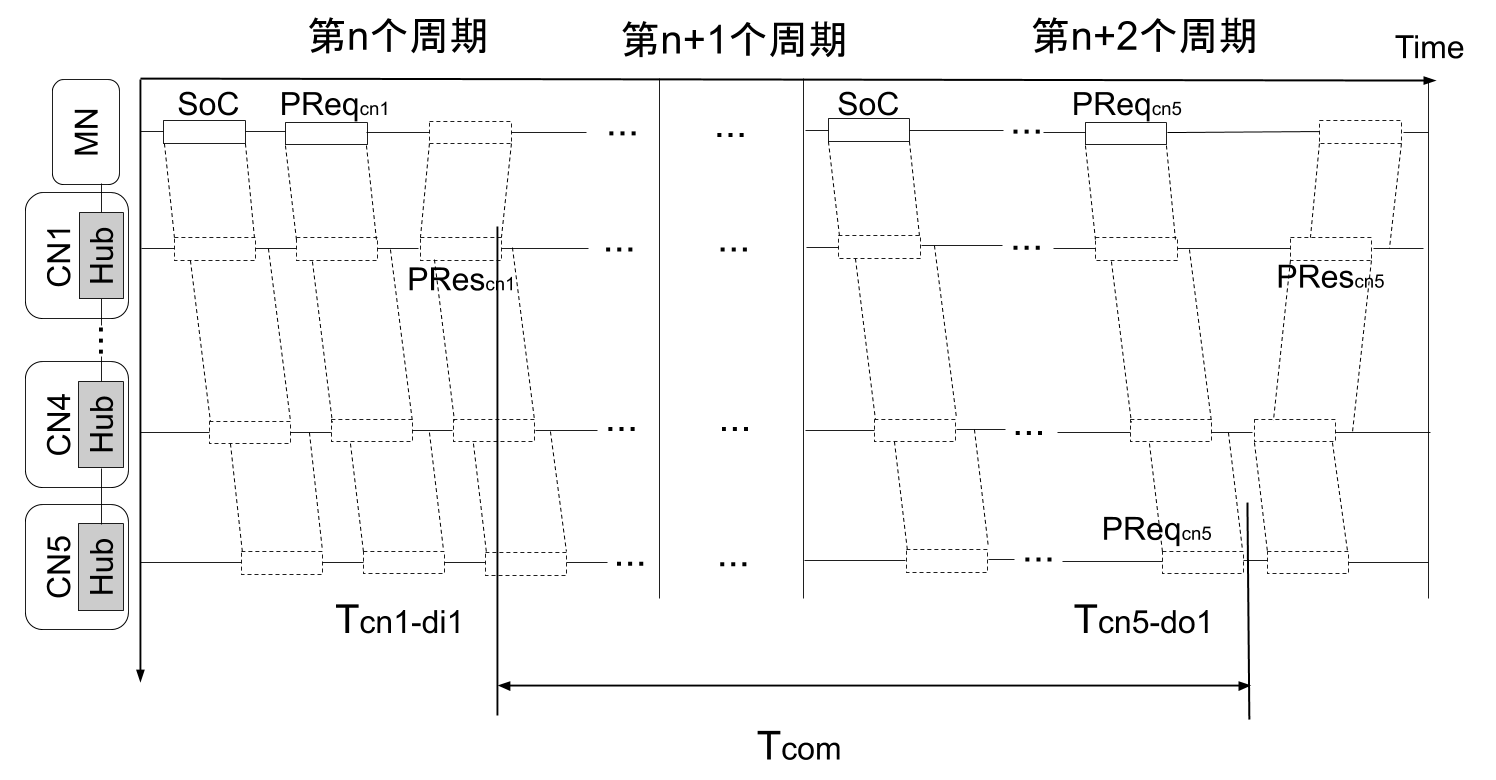
\includegraphics[width=\textwidth]{design2-response-process.png}
  \caption{方案2原型系统全局响应过程}
  \label{fig:design2-response-process}
\end{figure}

\begin{figure}[!htb]
  \centering
  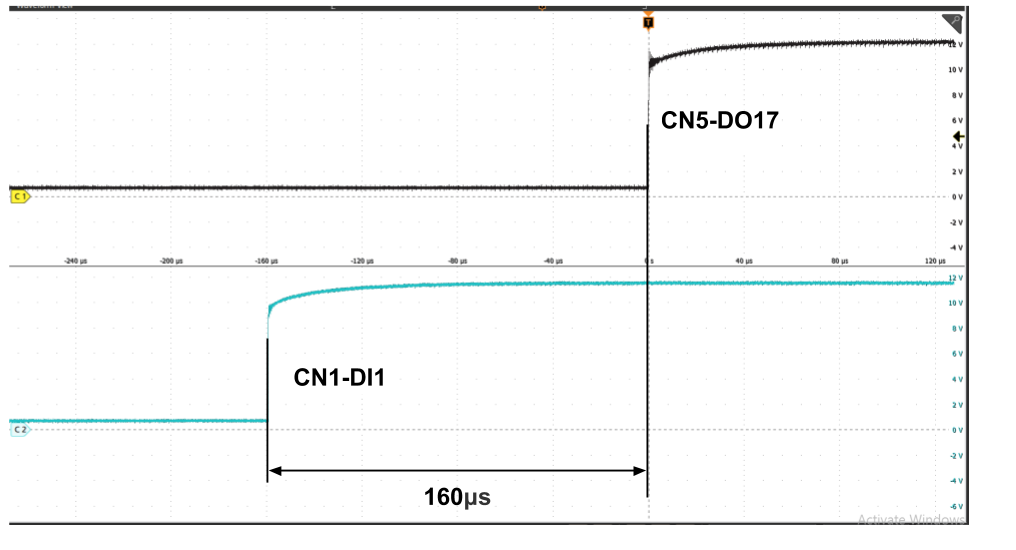
\includegraphics[width=\textwidth]{design2-response-time-result.png}
  \caption{方案2原型系统全局响应时间测试结果}
  \label{fig:design2-response-time-result}
\end{figure}

\subsection{主站响应时间测试}
主站的响应时间是指当主站收到来自从站的PRes数据帧到回复PReq数据帧的时间。主站响应时间直接影响系统的响应时间,主站响应时间与设备类型有关,方案1的主站采用的是基于x86运行Linux的pc,方案2采用的基于Zynq的主站控制器。如图~\ref{fig:design1-cycle-time-test}所示,相邻PRes数据帧和PReq数据帧之间时间差为主站响应时间($T_{r-mn}$)和PReq数据帧的传输时间($T_{F(PReq)}$之和。PReq数据帧长度为64Byte,采用千兆以太网传输,则$T_{F(PReq)}$为0.512$\mu$s。可得$T_{r-mn}$的计算结果如表~\ref{table:3.1}所示,基于Zynq控制器的响应时间平均值为1.865$\mu$s小于基于x86的pc16.296$\mu$s的响应时间,主站采用Zynq控制器来实现能更好的提升系统实时性能。

\begin{table}[hbt]
	\centering
	\caption{主站响应时间测试}
	\begin{tabular}{cccccc}
		\toprule
		主站设备类型 & 基于x86运行Linux的pc & 基于Zynq的控制器 \\
		\midrule
		响应时间平均值(μs) & 16.296 & 1.865 \\
		\bottomrule
	\end{tabular}
	\label{table:3.1}
\end{table}

\subsection{测试小结}
本节对方案1和方案2两种原型系统进行了性能测试,包括通信周期、系统响应时间和主站响应时间,根据测试结果,总结如下:

\begin{enumerate}
  \item 方案1原型系统可以在275$\mu$s周期下稳定运行,方案2原型系统可以稳定运行在50$\mu$s周期下。虽然两个原型系统站点数不同,但是如图~\ref{fig:design1-cycle-time-test}所示,方案1系统在完成第5个从站通信时已经耗时约为86$\mu$s,所以方案2原型系统的实时性优于方案1。
  \item 在响应时间的测试中,方案1从站控制器的光耦合器耗时为400$\mu$s,方案2从站控制器改用磁耦合器后,可将本地响应时间缩短至5$\mu$s。
  \item 方案1与方案2的主要差异在于主站设备类型的不同,方案1中基于Zynq的主站响应时间平均值为2.377$\mu$s远小于方案2中基于x86的pc的18.673$\mu$s。随着从站数量增加时,主站的响应延时会成倍增加,对系统实时性的影响会进一步放大。
  \item 方案2的原型系统在通信周期和响应时间等实时性能上优于方案1,但是由于原型系统从站数量的限制,很难再通过实测来评估更多节点系统的性能。所以,我们将采用理论计算和仿真模拟的方法对方案2架构下更大规模的系统进行性能评估。
\end{enumerate}

\section{理论计算POWERLINK通信周期}

\label{section:理论计算POWERLINK通信周期}
通信周期直接反应系统的实时性,决定了系统的响应时间,采用理论计算和仿真建模分析两种方法来对通信周期进行对比研究,可以为不同应用场合的技术方案设计提供依据。本节首先详细分析POWERLINK通信周期的时间组成,然后结合第\ref{section:原型系统性能测试}节中的实测数据来计算从站响应时间、HUB延时等通信参数,从而进一步完善理论计算方法,最后推导出通信周期的计算公式。

\subsection{等时同步阶段时间的理论计算}

\label{subsection:等时同步阶段时间的理论计算}

\begin{figure}[!htb]
  \centering
  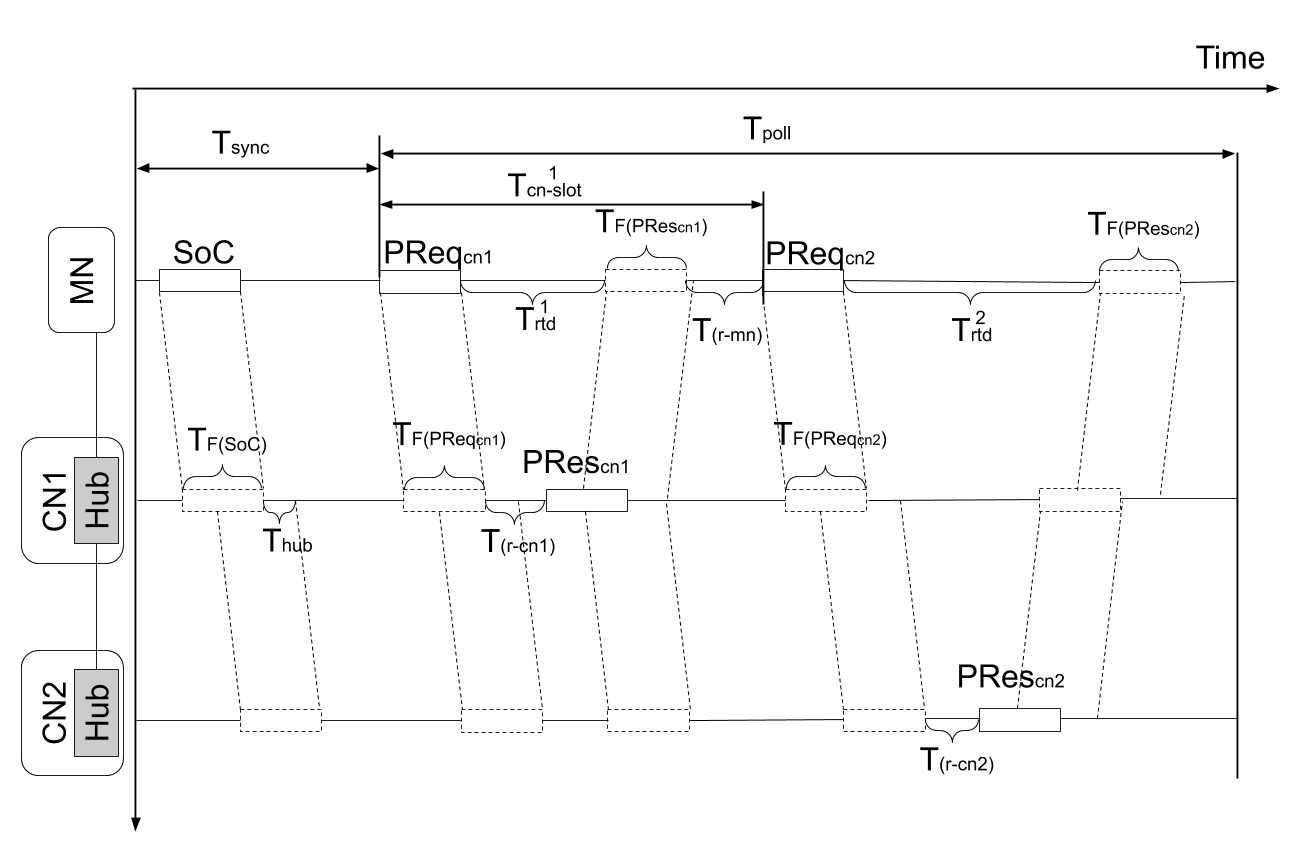
\includegraphics[width=\textwidth]{powerlink-communication-process.png}
  \caption{powerlink等时同步阶段通信过程}
  \label{fig:powerlink-communication-process}
\end{figure}

在POWERLINK通信周期中,等时同步阶段用来传输周期性的实时数据,占据了75\%以上的通信周期。图~\ref{fig:powerlink-communication-process}表示了一个基本POWERLINK网络的等时同步通信过程,该POWERLINK网络由一个主站和两个从站组成,各站点按照线型拓扑连接。等时同步阶段由同步阶段和轮询阶段组成,如公式~\ref{equation3}所示,其中$T_{ip}$代表等时同步阶段时间,$T_{sync}$和$T_{poll}$分别代表同步阶段和轮询阶段的时间。$T_{sync}$由公式~\ref{equation4}表示,$T_{F(SoC)}$为同步数据帧传输的时间。对于方案2的原型系统,SoC帧的大小为64Byte,采用千兆以太网传输,$T_{F(SoC)}$仅为0.512$\mu$s,$T_{W}$为等待从站接收并处理SoC帧的时间,从站是基于Zynq的控制器,处理速度极快。由图~\ref{fig:design2-cycle-time-test}所示,同步过程($T_{sync}$)在1$\mu$s以内可以完成,所以轮询阶段是是通信周期中耗时最长的阶段。

\begin{equation}
\label{equation3}
T_{ip}=T_{sync}+T_{poll}
\end{equation}

\begin{equation}
\label{equation4}
T_{sync}=T_{F(SoC)}+T_{W}
\end{equation}

轮询阶段时长($T_{poll}$)可由公式~\ref{equation5}表示,$T_{frames}$为轮询阶段中所有数据帧的传输时间,$T_{net}$为由所有网络组件造成的延时,网络组件包括主站、从站、HUB和网线。如图~\ref{fig:powerlink-communication-process}所示,PReq和PRes数据帧在每个从站时隙都会被发送,当主站和各从站的用户数据大小相等时,则PReq和PRes数据帧的传输时间相同均为$T_{F}$,$T_{frames}$可以用公式~\ref{equation6}表示。

\begin{equation}
\label{equation5}
T_{poll}=T_{frames}+T_{net}
\end{equation}

\begin{equation}
\label{equation6}
T_{frames}=\sum_{i=1}^n(T_{F(PReq)}^{i}+T_{F(PRes)}^{i})=2nT_{F}
\end{equation}
\begin{equation}
\label{equation7}
T_{net}=\sum_{i=1}^nT_{rtd}^{i}+nT_{r-mn}
\end{equation}

$T_{net}$由公式~\ref{equation7}表示,如图~\ref{fig:powerlink-communication-process}所示,$T_{rtd}^{i}$为主站在第i个从站时间间隙内的往返延时,$T_{r-mn}$为主站的响应时间。对于图~\ref{fig:powerlink-communication-process}所示的POWERLINK网络结构,$T_{rtd}^{1}$和$T_{rtd}^{2}$分别由公式~\ref{equation8}和~\ref{equation9}表示,其中$T_{c}$为网线传播延时,$T_{hub}$为从站控制器的HUB延时,$T_{r-cni}$为第i个从站的处理时间。根据公式~\ref{equation8}和~\ref{equation9},$T_{rtd}^{i}$可用公式~\ref{equation10}所示,因为从站设备类型相同,$T_{r-cni}$都等于$T_{r-cn}$。

\begin{equation}
\label{equation8}
T_{rtd}^{1}=2T_{c}+T_{hub}+T_{r-cn1}
\end{equation}

\begin{equation}
\label{equation9}
T_{rtd}^{2}=4T_{c}+3T_{hub}+T_{r-cn2}
\end{equation}

\begin{equation}
\label{equation10}
T_{rtd}^{i}=2iT_{c}+(2i-1)T_{hub}+T_{r-cn}
\end{equation}

\begin{equation}
\label{equation11}
\sum_{i=1}^ni=n(n+1)/2
\end{equation}

我们假设所有的从站设备类型相同且使用等长网线连接,即对于每个从站来说,参数$T_{c}$,$T_{hub}$和$T_{r-cn}$均相等。将公式~\ref{equation10}和公式~\ref{equation11}代入公式~\ref{equation7},可得公式~\ref{equation12},$T_{net}^{line}$为线性拓扑结构下所有网络组件造成的延时。

\begin{equation}
\begin{split}
\label{equation12}
T_{net}^{line}&=\sum_{i=1}^n[2iT_{c}+(2i-1)T_{hub}+T_{r-cn}]+nT_{r-mn}\\
&=n(n+1)T_{c}+n^2T_{hub}+n(T_{r-cn}+T_{r-mn})
\end{split}
\end{equation}

如图~\ref{fig:powerlink-communication-process}所示,$T_{poll}$为各从站的通信时隙$T_{cn-slot}^{i}$之和,$T_{poll}$也可以用公式~\ref{equation13}表示。根据图~\ref{fig:powerlink-communication-process}所示,$T_{cn-slot}^{i}$可用公式~\ref{equation14}表示。

\begin{equation}
\label{equation13}
T_{poll}^{i}=\sum_{i=1}^nT_{cn-slot}^{i}
\end{equation}

\begin{equation}
\label{equation14}
T_{cn-slot}^{i}=T_{F(PReq)}^{i}+T_{F(PRes)}^{i}+T_{rtd}^{i}+T_{r-mn}
\end{equation}

\subsection{通信参数的计算}

\begin{figure}[!htb]
  \centering
  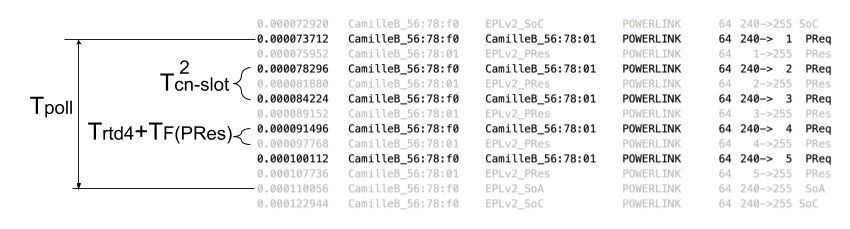
\includegraphics[width=\textwidth]{test-theory-powerlink.png}
  \caption{原型系统抓包结果}
  \label{fig:test-theory-powerlink}
\end{figure}

通过第\ref{section:原型系统性能测试}节中对方案2原型系统实测所得的数据,结合第\ref{subsection:等时同步阶段时间的理论计算}节中对等时同步阶段的理论分析,
计算出基于zynq控制器的$T_{hub}$、$T_{r-cn}$等参数,并推导出轮询阶段时长的计算公式。

对于方案2的原型系统,主站和每个从站的用户数据均为2Byte时,PReq和PRes数据帧的大小均为64Byte,$T_{F(PReq)}$等于$T_{F(PRes)}$,由~\ref{equation15}得相邻从站时隙的差值为$2T_{c}+2T_{hub}$,是个定值,表示从站时间间隙随着节点号的变大呈线性增长。如图~\ref{fig:test-theory-powerlink}所示,相邻两个PReq数据帧之间的时间差等于该从站时间间隙($T_{cn-slot}$),我们可以计算出每个从站的时间间隙,结果列于表~\ref{table:3.2}。图~\ref{fig:fit-line}为从站平均时间间隙散点图,我们添加了线性拟合趋势线,R平方值为1,表示拟合程度高,趋势线的可靠性高。拟合直线的函数斜率为1.3411等于$2T_{c}+2T_{hub}$,$T_{c}$为网线的延时,网线长度为2m,延时为(5ns/m),则$T_{hub}$为0.66$\mu$s。如图~\ref{fig:test-theory-powerlink}所示,相邻的PRes数据帧和PReq数据帧之间的时间差为$T_{rtd}^{i}$和$T_{F(PRes)}$之和,结合公式~\ref{equation10},可以计算得到$T_{r-cn}$的平均值为1.048$\mu$s。我们将一些重要通信参数的计算结果汇总列入表~\ref{table:3.2}中。

\begin{table}[hbt]
	\centering
	\caption{通信参数统计}
	\begin{tabular}{cccccc}
		\toprule
		主站响应时间($T_{r-mn}$) & 从站响应时间 ($T_{r-cn}$)& HUB延时 ($T_{hub}$)\\
		\midrule
		1.865μs & 1.048μs & 0.66μs\\
		\bottomrule
	\end{tabular}
	\label{table:3.2}
\end{table}

\begin{equation}
\begin{split}
\label{equation15}
T_{cn-slot}^{i+1}-T_{cn-slot}^{i}&=T_{rtd}^{i+1}-T_{rtd}^{i}\\
&=2T_{c}+2T_{hub}
\end{split}
\end{equation}

\begin{table}[hbtp]
	\centering
	\caption{从站时间间隙统计表:}
	\begin{tabular}{p{70 pt}p{70 pt}p{70 pt}p{70 pt}p{70 pt}}
		\toprule
		& Min & Max & Mean & Std.Dev\\
		\midrule
		$T_{cn-slot}^{1}$ & 4.56 & 4.584 & 4.572 & 0.0072\\
		$T_{cn-slot}^{2}$ & 5.90 & 5.94 & 5.91 & 0.0091\\
		$T_{cn-slot}^{3}$ & 7.25 & 7.3 & 7.26 & 0.0069\\
		$T_{cn-slot}^{4}$ & 8.66 & 8.59 & 8.607 & 0.0099\\
		$T_{cn-slot}^{5}$ & 9.91 & 9.98 & 9.929 & 0.0102\\
		\bottomrule
	\end{tabular}
	\\
	\footnotesize{所有数值均以$\upmu$s表示。}
	\label{table:3.2}
\end{table}

\begin{figure}[!htb]
  \centering
  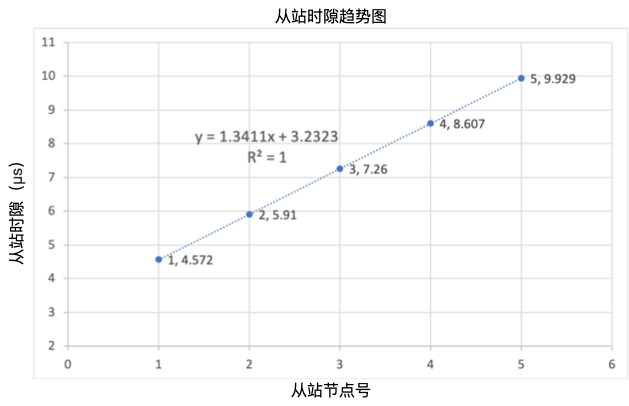
\includegraphics[width=\textwidth]{fit-line.png}
  \caption{从站时隙趋势图}
  \label{fig:fit-line}
\end{figure}

根据公式~\ref{equation5}、公式~\ref{equation6}和公示~\ref{equation12},并代入$T_{hub}$=0.66$\mu$s,$T_{r-cn}$=1.048$\mu$s,我们推导出基于zynq控制器的线性拓扑结构下POWERLINK网络等时同步阶段时长的公式为~\ref{equation16}。

\begin{equation}
\begin{split}
\label{equation16}
T_{poll}=&\sum_{i=1}^n(T_{F(PReq)}^{i}+T_{F(PRes)}^{i})+T_{net}^{line}\\
&=\sum_{i=1}^n(T_{F(PReq)}^{i}+T_{F(PRes)}^{i})+0.67n^{2}+2.923n
\end{split}
\end{equation}

\section{网络模拟}
通过理论计算的分析方法,我们得到了zynq控制器的响应时间、HUB延时等通信参数,并初步推导出了等时同步阶段时长的计算公式。为了对更大规模的POWERLINK方案进行准确可靠的评估,我们还发展了仿真建模的分析方法。POWERLINK网络仿真基于OMNet++网络模拟器展开,我们首先建立了支持千兆POWERLINK通信的节点模型,然后通过对原型系统进行仿真来验证仿真建模分析方法的可行性,最后通过仿真建模的分析方法对大规模的POWERLINK方案进行性能评估。

OMNeT++(Objective Modular Network Testbed in C++)是一个开源可扩展的、模块化、基于组件的C++仿真库和框架,主要用于构建网络仿真器。作为面向对象的离散事件仿真器,OMNeT++主要用于通信网络和分布式系统的仿真。OMNeT++的主要组成部分如下:

\begin{enumerate}
  \item 仿真内核库:OMNeT++提供的仿真类库代码;
  \item 网络拓扑描述文件:由NED语言编写的文件,既可以用来描述网络拓扑结构,又可以通过参数、门、信道连接、简单模块等来定义复杂模块;
  \item 消息定义文件:用于定义数据报文格式;
  \item 简单模块定义文件:简单模块的行为定义文件,包括C++编写的*.cc文件和*.h
  \item 用户接口:该接口用于仿真运行时的测试,演示等工作。
\end{enumerate}

在使用OMNeT++建模中,最常使用的就是INET框架。INET框架是开源的OMNeT++的标准协议模型库,对应OMNeT的各种新版本INET框架还在不断更新中,INET框架包含了常用的多种有线和无线协议的模型,具体到各种物理层模型、应用层模型等。在POWERLINK仿真建模中,我们使用的是OMNeT++4.6版本搭配inet-2.6-b673687版本。

\subsection{POWERLINK通信节点建模}

\begin{figure}[!htb]
  \centering
  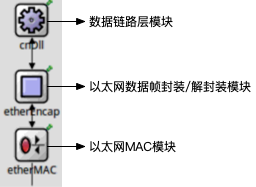
\includegraphics[width=0.6\textwidth]{powerlink-model.png}
  \caption{POWERLINK通信节点模型}
  \label{fig:powerlink-model}
\end{figure}
基于OMNeT++仿真平台,我们对POWERLINK主站和从站进行了建模。节点模型如图~\ref{fig:powerlink-model}所示,由以下三个模块组成:

\begin{enumerate}
  \item 以太网MAC模块:采用INET框架下的标准以太网MAC模块,支持千兆以太网通信;
  \item 以太网数据帧封装/解封装模块:采用INET框架下的EtherEncap模块,用于EthernetII数据帧的封装和解封装;
  \item 数据链路层模块:按照POWERLINK的SCNM机制定义了模块行为。
\end{enumerate}

除了对通信节点建模之外,还定义了FPGAHUB模块用于数据帧的转发,采用INET框架下的Eth1G千兆以太网模块用于连接各节点,在.msg文件中定义四种POWERLINK数据帧结构。

\subsection{建立原型系统仿真模型}

\begin{figure}[!htb]
  \centering
  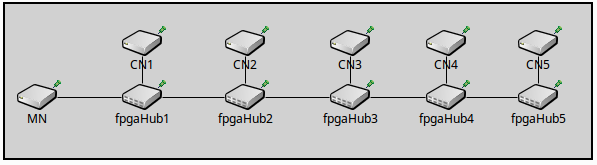
\includegraphics[width=\textwidth]{5node-model-omnet.png}
  \caption{原型系统模型}
  \label{fig:5node-model-omnet}
\end{figure}

为了验证通信节点模型的准确性和仿真建模方法的可行性,我们首先对方案2原型系统进行了建模。原型系统的模型如图~\ref{fig:5node-model-omnet}所示,节点数和拓扑结构均与原型系统保持一致,相邻节点之间通过2m长的网线相连,节点之间的通信基于千兆POWERLINK。对于原型系统中从站控制器的模拟,我们采用从站通信节点模块加上FPGA HUB模块来实现,两模块间传输延时设置为0$\mu$s。除此之外,为了准确模拟原型系统,我们采用原型系统中的实测参数对系统模型进行了配置,配置文件包括xdcMN.xml和omnetpp.ini。xdcMN.xml文件中配置了主站对各从站发送数据的大小(PReqActPayload)和各从站被分配的通信时隙(PResTimeout),其中各从站的通信时隙通过公式~\ref{equation14}计算得到,公式中相关参数使用表~\ref{table:3.2}中的数据,具体配置如下:
\begin{lstlisting}
<Nodes>
  <Node NodeId="1" PResTimeout="4617ns" PReqActPayload="2byte" />
  <Node NodeId="2" PResTimeout="5958ns" PReqActPayload="2byte" />
  <Node NodeId="3" PResTimeout="7299ns" PReqActPayload="2byte" />
  <Node NodeId="4" PResTimeout="8640ns" PReqActPayload="2byte" />
  <Node NodeId="5" PResTimeout="9981ns" PReqActPayload="2byte" />
</Nodes>
\end{lstlisting}

omnetpp.ini仿真配置文件包括了对系统通信周期、各从站节点号和响应数据大小、HUB延时的设定,具体内容如下:

\begin{lstlisting}
[Config EPLBase]

# 通信周期设置
**.MN.mnDll.cycleLenMean = 50us

# 各从站节点号和pres数据大小设定
**.CN1.cnDll.nodeId = 1
**.CN1.cnDll.presActPayload = 2
**.CN2.cnDll.nodeId = 2
**.CN2.cnDll.presActPayload = 2
**.CN3.cnDll.nodeId = 3
**.CN3.cnDll.presActPayload = 2
**.CN4.cnDll.nodeId = 4
**.CN4.cnDll.presActPayload = 2
**.CN5.cnDll.nodeId = 5
**.CN5.cnDll.presActPayload = 2

# FPGA HUB延时设定
**.hubDelayMean = 0.66us

[Config EPL4StdSettings]
**.MN.mnDll.xdcMN = xmldoc("xdcMN.xml")
\end{lstlisting}

模拟过程持续了大约3000个POWERLINK通信周期。等时同步阶段的概率密度分布绘制在图~\ref{fig:iso-time-density-5cn-model}中,该图表明大多数情况下的等时同步阶段时长为37.2$\mu$s,最大抖动不超过30ns。
\begin{figure}[!htb]
  \centering
  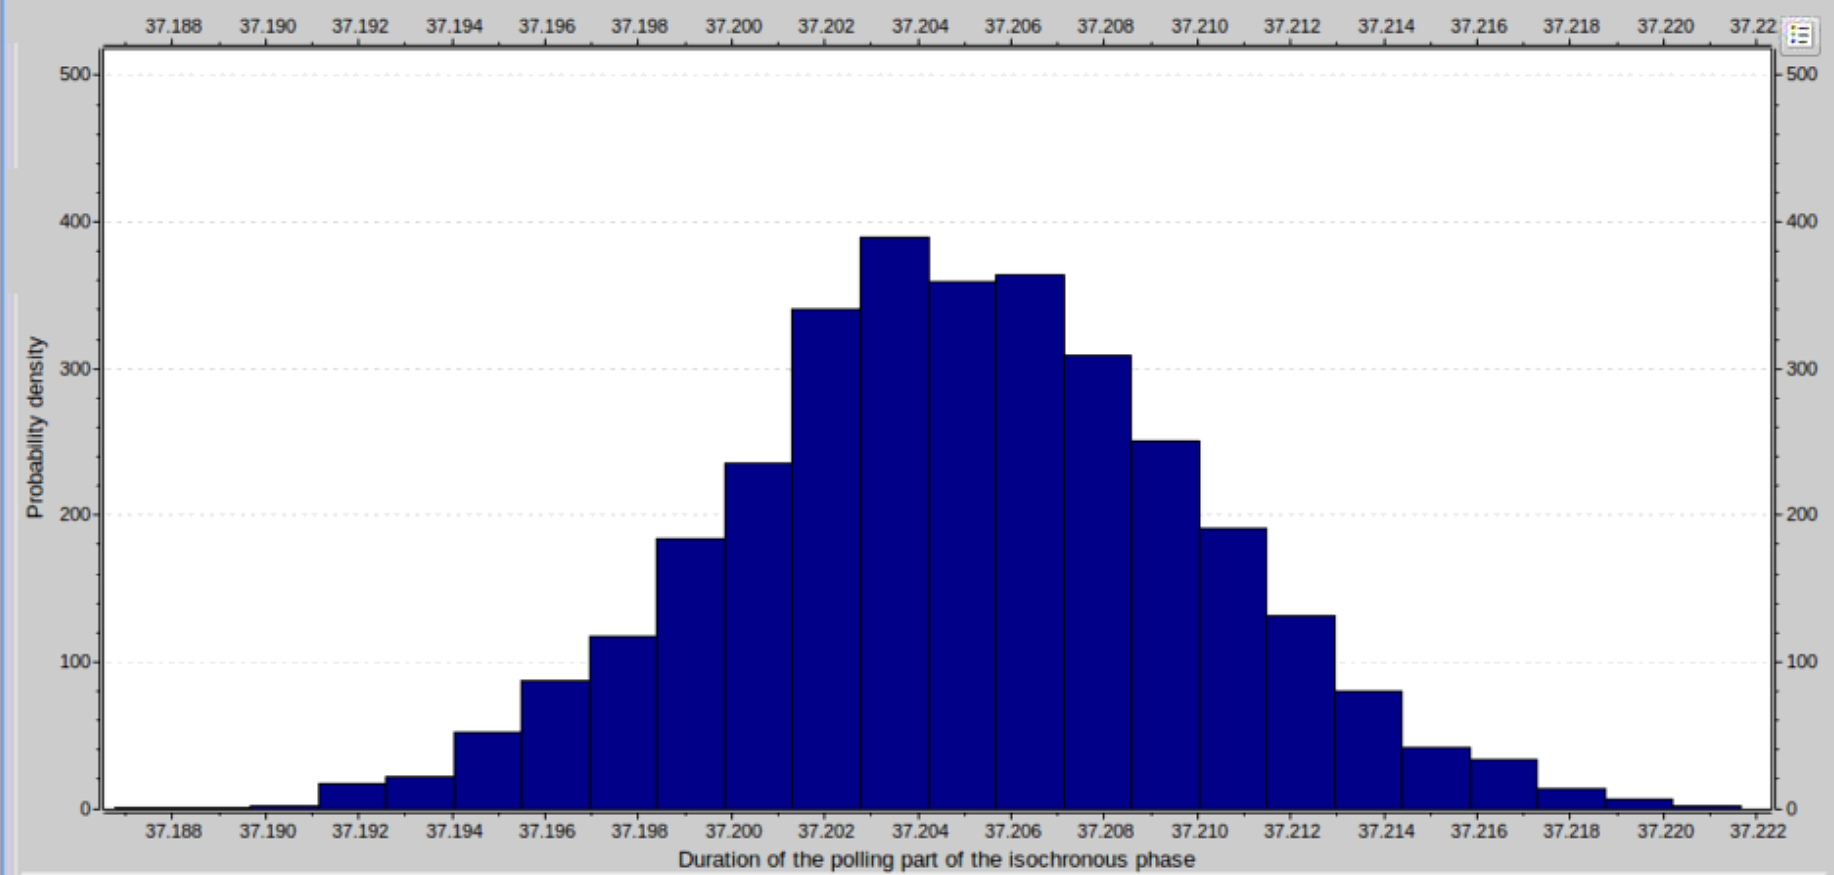
\includegraphics[width=\textwidth]{iso-time-density-5cn-model.png}
  \caption{原型系统模型轮询阶段的概率密度分布}
  \label{fig:iso-time-density-5cn-model}
\end{figure}

对于方案2原型系统,我们通过实测、理论计算和仿真模拟三种方式得到轮询阶段的时长,其中实测结果如图~\ref{fig:test-theory-powerlink}中$T_{poll}$所示,理论计算结果通过公式~\ref{equation16}得出,具体结果如表~\ref{table:3.2}所示。较之实测值,理论计算和仿真模拟的两种方法对轮询阶段时长的计算误差在1$\mu$s以内,1$\mu$s误差对于50$\mu$s的通信周期来说影响非常小,所以理论计算和仿真模拟的两种方法可以准确的估算轮询阶段的时长。考虑到同步阶段不足1$\mu$s的耗时以及等时同步阶段在POWERLINK周期中至少75\%的占比,我们可以估算出POWERLINK通信周期。

\begin{table}[hbt]
	\centering
	\caption{主站响应时间测试}
	\begin{tabular}{cccccc}
		\toprule
		 & 实测 & 理论计算 & 模拟仿真 \\
		\midrule
		轮询阶段时长平均值(μs)& 36.312 & 36.485   & 37.2\\
		\bottomrule
	\end{tabular}
	\label{table:3.3}
\end{table}

\section{分析评估多节点分布式系统的实时性能}

在原型系统的研究基础上,我们采用理论计算和仿真模拟的方法对更大规模的POWERLINK系统进行了实时性能评估。该系统架构如图~\ref{fig:10cn-powerlink-arch}所示,POWERLINK网络由1个主站和10个从站组成,每个从站按节点号从小到大的顺序依次相连成线型拓扑结构,各节点的设备类型和配置与原型系统中各节点相同。由于IOC负责监控POWERLINK网络中各节点状态,并不参与POWERLINK通信,所以系统实时性能即是POWERLINK网络部分的实时性能。

\begin{figure}[!htb]
  \centering
  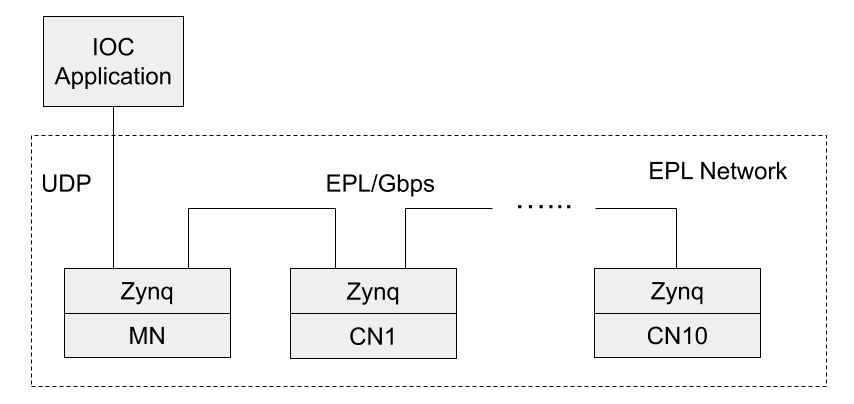
\includegraphics[width=\textwidth]{10cn-powerlink-arch.png}
  \caption{10节点POWERLINK系统架构图}
  \label{fig:10cn-powerlink-arch}
\end{figure}

基于第\ref{section:理论计算POWERLINK通信周期}节中对通信周期的分析,我们可以直接采用公式~\ref{equation10}来计算轮询阶段的时长,其中节点数n=10,PReq和PRes数据帧长度均为64Byte,$T_{F(PReq)}$和$T_{F(PRes)}$相等均为0.512$\mu$s,将以上数值代入公式~\ref{equation16},可得轮询阶段阶段时长为106.47$\mu$s。考虑到同步阶段不足1$\mu$s的耗时以及等时同步阶段在POWERLINK周期中至少75\%的占比,我们可以估算出此系统POWERLINK通信周期为143.293$\mu$s。

\begin{figure}[!htb]
  \centering
  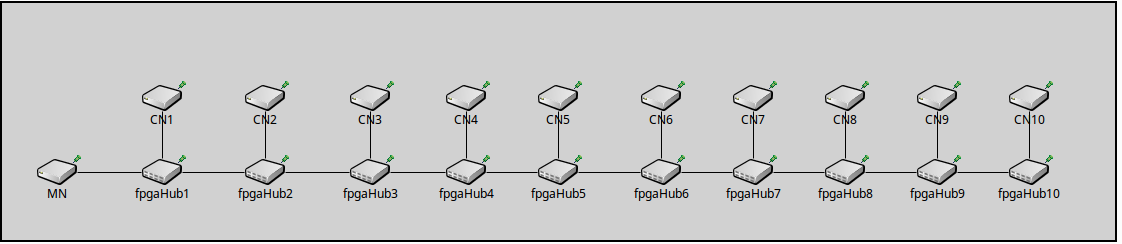
\includegraphics[width=\textwidth]{10node-model-omnet.png}
  \caption{10节点POWERLINK系统模型}
  \label{fig:10node-model-omnet}
\end{figure}

基于OMNeT++仿真平台,我们对系统进行了建模,模型如图~\ref{fig:10node-model-omnet}所示。较之原型系统模型新增了6-10号从站,新增从站被分配的通信时隙(PResTimeout)通过公式~\ref{equation14}计算得到,公式中相关参数使用表~\ref{table:3.2}中的数据,具体配置如下:
\begin{lstlisting}
<Nodes>
  <Node NodeId="1" PResTimeout="4617ns" PReqActPayload="2byte" />
  <Node NodeId="2" PResTimeout="5958ns" PReqActPayload="2byte" />
  <Node NodeId="3" PResTimeout="7299ns" PReqActPayload="2byte" />
  <Node NodeId="4" PResTimeout="8640ns" PReqActPayload="2byte" />
  <Node NodeId="5" PResTimeout="9981ns" PReqActPayload="2byte" />
  <Node NodeId="6" PResTimeout="11328ns" PReqActPayload="2byte" />
  <Node NodeId="7" PResTimeout="12669ns" PReqActPayload="2byte" />
  <Node NodeId="8" PResTimeout="14010ns" PReqActPayload="2byte" />
  <Node NodeId="9" PResTimeout="15351ns" PReqActPayload="2byte" />
  <Node NodeId="10" PResTimeout="16692ns" PReqActPayload="2byte" />
</Nodes>
\end{lstlisting}

模拟过程持续了大约2000个POWERLINK通信周期。等时同步阶段的概率密度分布绘制在图~\ref{fig:iso-time-density-5cn-model}中,该图表明大多数情况下的等时同步阶段时长为106.8$\mu$s,最大抖动不超过40ns。考虑到同步阶段不足1$\mu$s的耗时以及等时同步阶段在POWERLINK周期中至少75\%的占比,我们可以估算出此系统POWERLINK通信周期为143.733$\mu$s。

\begin{figure}[!htb]
  \centering
  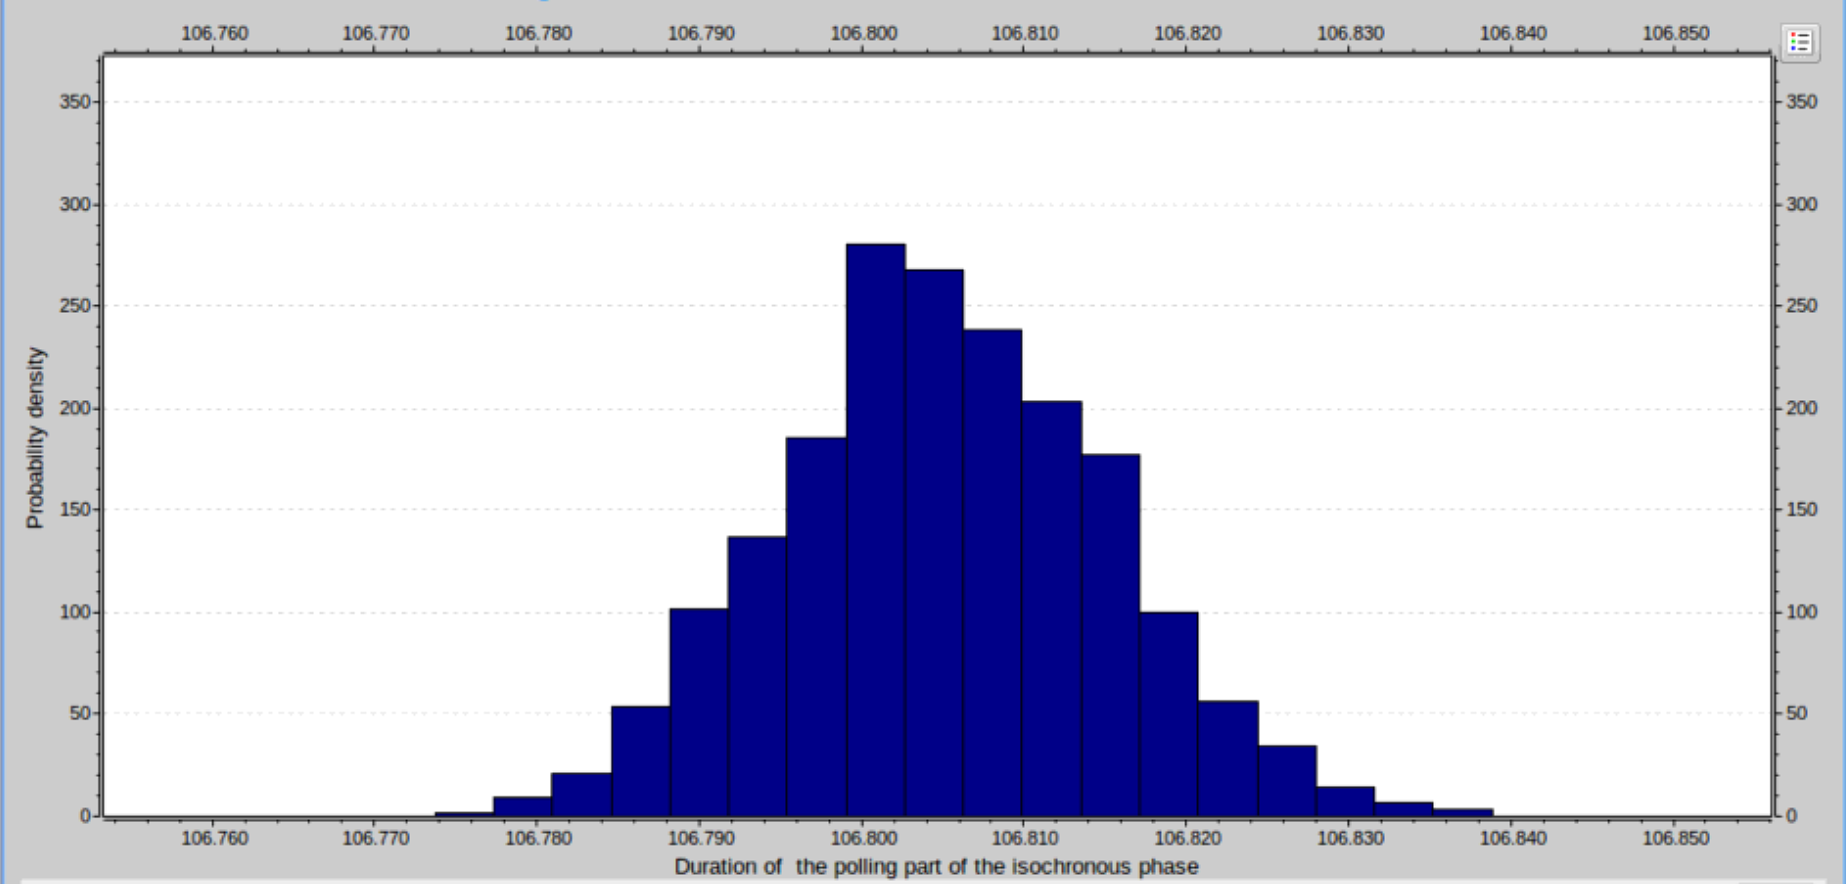
\includegraphics[width=\textwidth]{10node-model-density.png}
  \caption{10节点系统模型轮询阶段的概率密度分布}
  \label{fig:10node-model-density}
\end{figure}



